\RequirePackage{fix-cm}
\RequirePackage{cmap}
\documentclass[aps,pra,reprint,nofootinbib,floatfix,longbibliography]{revtex4-2}

\usepackage[T1]{fontenc}
\usepackage[utf8]{inputenc}
\input{glyphtounicode}
\pdfgentounicode=1
\usepackage{amsmath,amsthm,mathtools}
\usepackage{newtxtext}
\usepackage{newtxmath}
\DeclareMathAlphabet{\mathcal}{OMS}{cmsy}{m}{n}
\usepackage{bm}
\usepackage{microtype}
\emergencystretch=1.5em
\usepackage{graphicx}
\usepackage{booktabs}
\usepackage{xcolor}
\usepackage[colorlinks=true,linkcolor=blue!70!black,citecolor=blue!70!black,urlcolor=blue!70!black]{hyperref}

% Theorem environments compatible with revtex4-2
\newtheorem{theorem}{Theorem}
\newtheorem{proposition}{Proposition}
\newtheorem{lemma}{Lemma}
\newtheorem{corollary}{Corollary}
\theoremstyle{remark}
\newtheorem{remark}{Remark}

% Mathematical macros
\newcommand{\braket}[2]{\langle #1 | #2 \rangle}
\newcommand{\ket}[1]{| #1 \rangle}
\newcommand{\bra}[1]{\langle #1 |}
\newcommand{\norm}[1]{\lVert #1 \rVert}
\newcommand{\abs}[1]{\lvert #1 \rvert}

\begin{document}

\title{Overcompleteness and Continuous Frame Properties of Physical Perfect Vortex Beams.\\I. Operator Theory and Laguerre--Gaussian Expansion}

\author{Sebasti\'an Ayala}
\email{ayala.phys.ds@gmail.com}
\homepage{https://orcid.org/0009-0003-7348-3883}
\affiliation{Independent Researcher, Cauquenes, Chile}

\date{November 21, 2026}

\begin{abstract}
Physical perfect optical vortex beams (PVBs) possess an annular intensity profile of finite half-width $w > 0$ whose ring radius $R > 0$ is nominally independent of the orbital angular momentum (OAM) topological charge $l \in \mathbb{Z}$. Here, we establish their rigorous operator-theoretic foundation as continuous Hilbert frames on transverse wavefields. While azimuthal OAM sectors decouple into strictly orthogonal subspaces ($\delta_{l,l'}$), continuous radial nonorthogonality ($\gamma_l(R,R') \in (0,1)$, governed at large radii by the $l$-independent Gaussian law $e^{-(R-R')^2/(2w^2)}$) induces a continuous frame operator $S_w$ acting as an isotropic Gaussian convolution $G_w * \cdot$, yielding an optimal Bessel upper bound $B = 1$ and a vanishing global lower bound $A = 0$ on unconstrained $L^2(\mathbb{R}^2)$. Restricted to any paraxial Paley--Wiener bandlimited subspace $\mathcal{H}_{k_{\max}}$, projected physical PVBs form a stable continuous frame with sharp bounds $A(w,k_{\max}) = \exp(-w^2 k_{\max}^2/2)$ and $B = 1$. We construct the Tikhonov-regularized canonical dual frame $S_{w,\alpha_{\mathrm{reg}}}^{-1} = (S_w^2 + \alpha_{\mathrm{reg}}\mathbb{I})^{-1}S_w$ and prove that its spectral deconvolution noise gain peaks at $(2\sqrt{\alpha_{\mathrm{reg}}})^{-1}$ at spatial frequency $k_{\mathrm{peak}} = w^{-1}\sqrt{\ln(1/\alpha_{\mathrm{reg}})}$. Extending finite-width PVB projections beyond zero radial order, we prove an exact $(p+1)$-term closed-form expansion $c_{l,p}(R)$ for arbitrary Laguerre--Gaussian ($\mathrm{LG}_{p,l}$) eigenmodes ($p \ge 0$), establish both the exact $p = 0$ fidelity threshold and the generalized nodal Rayleigh limit $w_{\mathrm{crit}} \approx 0.573\,w_0/\sqrt{2p+\abs{l}+1}$ ($p \ge 1$), and prove that unit-normalized discrete radial Gram matrices converge monotonically to a bounded Jacobi-theta Toeplitz spectrum ($\kappa(\gamma) = 1.645$ at $\Delta R = 2.0\,w$, $17.36\,\mathrm{dB}$ adjacent power isolation). Classical and quantum photonic applications of this framework are presented in the companion paper (Paper~II).
\end{abstract}

\maketitle

\section{Introduction}
\label{sec:intro}

Structured paraxial wavefields carrying orbital angular momentum (OAM) have become foundational across classical and quantum optics since Allen \emph{et al.} showed that beams with helical phase $\exp(il\phi)$ carry $l\hbar$ of OAM per photon~\cite{Allen1992,Siegman1986,Padgett2011,Erhard2018}. In the standard orthonormal Laguerre--Gaussian ($\mathrm{LG}_{p,l}$) basis of waist $w_0$, however, the second-moment root-mean-square (RMS) beam radius expands with radial node number $p \in \mathbb{Z}_{\ge 0}$ and azimuthal charge $l \in \mathbb{Z}$ as $r_{\mathrm{rms}} = w_0\sqrt{2p+\abs{l}+1}$~\cite{Allen1992,Siegman1986} (while for $p = 0$ and $\abs{l} \ge 1$, the peak intensity ring radius scales as $r_{\mathrm{peak}} = w_0\sqrt{\abs{l}/2}$). To decouple annular geometry from topological charge, Ostrovsky \emph{et al.}~\cite{Ostrovsky2013} and Vaity and Rusch~\cite{Vaity2015} introduced the perfect optical vortex beam (PVB). In its singular Dirac-delta idealization, $\Phi_{l,R}^{\mathrm{ideal}}(r,\phi) = (2\pi)^{-1/2} R^{-1}\delta(r-R)e^{il\phi}$ satisfies $\braket{\Phi_{l,R}^{\mathrm{ideal}}}{\Phi_{l',R'}^{\mathrm{ideal}}} = \delta_{l,l'} R^{-1}\delta(R-R')$ under the polar radial measure $R\,dR$ [equivalently $(2\pi R)^{-1/2}\delta(r-R)e^{il\phi}$ with $\delta_{l,l'}\delta(R-R')$ under unweighted $dR$], forming a generalized orthonormal basis inside the distributional dual of a Gel'fand rigged Hilbert space~\cite{Gelfand1964}, whereas every physical realization carries a finite annular half-width $w > 0$ and finite transverse norm~\cite{Vaity2015,Reddy2016}.

Crucially, because the azimuthal harmonics $\{e^{il\phi}/\sqrt{2\pi}\}_{l\in\mathbb{Z}}$ form an exact orthonormal basis of $L^2(S^1)$ at any fixed radius $R$, nonorthogonality and overcompleteness in physical PVBs arise exclusively along the continuous radial parameter $R \in (0,\infty)$ within each fixed-$l$ sector. Recently, Ferreira \emph{et al.}~\cite{Ferreira2026} (Appendix~D) noted that finite-width PVBs fail radial orthogonality and induce Gaussian spatial smoothing, evaluating the radial projection overlap solely for zero-node modes ($p = 0$) while leaving arbitrary radial orders $p \ge 1$ and global operator inversion unresolved. Three foundational theoretical questions consequently remained open: (i) how finite-width PVBs are classified in continuous Hilbert frame theory~\cite{Duffin1952,Daubechies1990,Ali1993,Christensen2016} relative to orthogonal $\mathrm{LG}_{p,l}$ bases and Glauber coherent states~\cite{Klauder1985,Perelomov1986,Gazeau2009}; (ii) how sharp lower frame bounds are recovered on bandlimited optical subspaces and stabilized via canonical dual regularization; and (iii) whether an exact finite closed-form expansion $c_{l,p}(R)$ exists for all $\mathrm{LG}_{p,l}$ modes ($p \ge 0$) together with rigorous radial washout criteria and discrete Gram conditioning bounds.

Here we resolve all three theoretical questions in self-contained operator form, while deferring classical and quantum photonic protocols (noisy modal deconvolution, waveguide coupling, turbulent spatial filtering, multi-plane quantum tomography, and entangled aperture invariance) to the companion paper (Paper~II)~\cite{AyalaPaperII}. Methodologically, this two-part study was executed under a strict Human-in-the-Loop (HITL) scientific protocol~\cite{Krenn2022,Birhane2023,Messeri2024,Chandra2026TheoPhysEval,Thorp2023Science,COPE2023AI}: all physical questions, Hilbert-space domain restrictions ($L^2(\mathbb{R}^2)$ versus $\mathcal{H}_{k_{\max}}$), and frame-versus-state scaling conventions were originated and audited by the human author, while symbolic hypergeometric reductions and arbitrary-precision quadrature checks were accelerated with generative reasoning tooling as detailed in the Acknowledgments.

The remainder of this paper is organized as follows. Section~\ref{sec:pvb_formation} establishes our frame-versus-state scaling convention, dimensional homogeneity, differential radial peak shift (Sec.~\ref{subsec:pvb_def}), and $2f$ Bessel--Gauss Fourier generation and propagation regimes (Sec.~\ref{subsec:generation_bridge}). Section~\ref{sec:frame_theory} proves azimuthal--radial decoupling (Sec.~\ref{subsec:decoupling}), the optimal Bessel bound $B = 1$ and Gaussian convolution kernel (Sec.~\ref{subsec:frame_operator}), and sharp Paley--Wiener frame bounds (Sec.~\ref{subsec:paley_wiener}). Section~\ref{sec:properties} derives the Tikhonov-regularized canonical dual and its noise-gain peak (Sec.~\ref{subsec:tikhonov_dual} and Appendix~\ref{app:tikhonov_toeplitz}), the exact $(p+1)$-term $\mathrm{LG}_{p,l}$ expansion (Sec.~\ref{subsec:lg_expansion} and Appendix~\ref{app:lg_expansion}), the generalized radial Rayleigh criterion (Sec.~\ref{subsec:nodal_washout}), and discrete radial Gram conditioning (Sec.~\ref{subsec:gram_sampling}). Section~\ref{sec:conclusions} summarizes our conclusions.

\section{Physical PVBs: Conventions, Asymptotics, and Paraxial Generation}
\label{sec:pvb_formation}

\subsection{Complex Field, Scaling Convention, and Differential Radial Shift}
\label{subsec:pvb_def}

In cylindrical coordinates $\mathbf{r} = (r,\phi)$ at the focal waist plane $z = 0$, a physical PVB of topological charge $l \in \mathbb{Z}$, ring radius $R > 0$, and annular half-width $w > 0$ has transverse complex envelope~\cite{Ostrovsky2013,Vaity2015}
\begin{equation}
\Phi_{l,R}(r,\phi) = C_0 e^{il\phi} \exp\!\left(-\frac{r^2 + R^2}{w^2}\right) I_{\abs{l}}\!\left(\frac{2Rr}{w^2}\right),
\label{eq:pvb_mode}
\end{equation}
where $I_{\abs{l}}$ denotes the modified Bessel function of the first kind ($I_l(x) = I_{\abs{l}}(x)$ for $l \in \mathbb{Z}$) and
\begin{equation}
C_0 = \frac{1}{w^2}\sqrt{\frac{2}{\pi}}.
\label{eq:C0_norm}
\end{equation}
In physical length units $\ell_0$, $C_0$ and $\Phi_{l,R}$ carry dimensions $[\mathrm{length}^{-2}]$ and are \emph{not} unit-$L^2(\mathbb{R}^2)$-normalized states; rather, Eq.~\eqref{eq:C0_norm} is the natural resolution-of-identity frame scaling that fixes the optimal upper frame bound $B = 1$ under the polar radial measure $d\mu(l,R) = R\,dR$ (which carries dimensions $[\mathrm{length}^2]$). Specifically, denoting the transverse $L^2(\mathbb{R}^2)$ norm by $\norm{\psi}_{L^2} \equiv \norm{\psi}_{L^2(\mathbb{R}^2)} = (\int_{\mathbb{R}^2}\abs{\psi(\mathbf{r})}^2\,d^2\mathbf{r})^{1/2}$ (while writing $\norm{\cdot}_{\mathcal{H}}$ for general Hilbert spaces and $\norm{\cdot}$ for operator norms), for any wavefield $\psi \in L^2(\mathbb{R}^2)$ of unit dimensionless norm $\norm{\psi}_{L^2}^2 = 1$ ($[\psi] = [\mathrm{length}^{-1}]$), the analysis projection $\braket{\Phi_{l,R}}{\psi} = \int_{\mathbb{R}^2}\Phi_{l,R}^*(\mathbf{r})\psi(\mathbf{r})\,d^2\mathbf{r}$ carries dimensions $[\Phi_{l,R}^*][\psi][d^2\mathbf{r}] = [\mathrm{length}^{-1}]$, so both $\int_0^\infty R\,dR\,\abs{\braket{\Phi_{l,R}}{\psi}}^2$ and the frame operator $S_w$ are strictly dimensionless without requiring artificial unitless coordinates. Meanwhile, the squared $L^2(\mathbb{R}^2)$ norm of an individual frame vector is $\norm{\Phi_{l,R}}_{L^2}^2 = w^{-2} e^{-R^2/w^2} I_{\abs{l}}(R^2/w^2) < w^{-2}$ (for example, $\norm{\Phi_{l=1,\,R=2\ell_0}}_{L^2}^2 = 0.3894\,\ell_0^{-2} \neq 1$ at $w = 0.5\,\ell_0$).

\emph{Convention.} Throughout this paper, the continuous frame elements are the unnormalized modes $\{\Phi_{l,R}\}$ of Eq.~\eqref{eq:pvb_mode}, whereas the unit-$L^2$-normalized states $\psi_{l,R} = \Phi_{l,R}/\norm{\Phi_{l,R}}_{L^2}$ (carrying dimensions $[\mathrm{length}^{-1}]$) are used when evaluating normalized single-channel overlaps and discrete channel Gram matrices (Sec.~\ref{subsec:gram_sampling}). Accordingly, the continuous frame bounds in Lemma~\ref{lem:bessel_upper} and Theorem~\ref{thm:pw_bounds} refer strictly to $\{\Phi_{l,R}\}$, whereas the discrete multi-ring conditioning analysis in Sec.~\ref{subsec:gram_sampling} uses $\gamma_l(R,R') = \braket{\psi_{l,R}}{\psi_{l,R'}}$. We restrict the annular index set to $R > 0$: at the endpoint $R = 0$, $\Phi_{l,0} \equiv 0$ identically for all $l \neq 0$, while $l = 0$ reduces to the on-axis Gaussian $\Phi_{0,0}(r) = C_0 e^{-r^2/w^2}$ with $\norm{\Phi_{0,0}}_{L^2}^2 = 1/w^2$, a singleton of zero $R\,dR$ measure.

Applying Hankel's large-argument expansion $I_{\abs{l}}(x) = (2\pi x)^{-1/2} e^x [1 - (4l^2 - 1)/(8x) + \mathcal{O}(x^{-2})]$ with $x = 2Rr/w^2$ and $C_0 = w^{-2}\sqrt{2/\pi}$, Eq.~\eqref{eq:pvb_mode} approaches the thin-annulus Gaussian ring~\cite{Ferreira2026}
\begin{equation}
\Phi_{l,R}(r,\phi) \approx \frac{e^{il\phi}}{w\sqrt{2\pi^2 Rr}} \exp\!\left[-\frac{(r - R)^2}{w^2}\right],
\label{eq:pvb_thin_ring}
\end{equation}
carrying exact dimensions $[\mathrm{length}^{-2}]$ uniformly for $r \sim R \gg w$ and $\abs{l} \ll 2R/w$ (equivalently $l^2 \ll 4Rr/w^2$). Near the optical axis ($r \to 0$), however, Eq.~\eqref{eq:pvb_thin_ring} diverges unphysically as $r^{-1/2}$ whereas Eq.~\eqref{eq:pvb_mode} vanishes regularly as $r^{\abs{l}}$; even at $R/w = 4$ and $l = 4$ ($x = 32$), the leading-order approximation incurs a $28.4\%$ relative error. Extremizing $\abs{\Phi_{l,R}(r)}^2$ yields the exact transcendental condition $r_{\mathrm{peak}}(l) = R\,I'_{\abs{l}}(x_{\mathrm{peak}})/I_{\abs{l}}(x_{\mathrm{peak}})$ with $x_{\mathrm{peak}} = 2R r_{\mathrm{peak}}(l)/w^2$. Using the logarithmic derivative expansion $I'_{\abs{l}}(x)/I_{\abs{l}}(x) = 1 - (2x)^{-1} + (4l^2 - 1)/(8x^2) + \mathcal{O}(x^{-3})$ and substituting $x_{\mathrm{peak}}^{-1} = [w^2/(2R^2)][1 + w^2/(4R^2) + \mathcal{O}(w^4/R^4)]$ self-consistently into $-(2x_{\mathrm{peak}})^{-1}$ shifts the quadratic coefficient to $(4l^2 - 1)/8 - 1/4 = (4l^2 - 3)/8$,\footnote{Specifically, the leading term is $-(2x_{\mathrm{peak}})^{-1} \approx -w^2/(4R^2)$, while the first self-consistent correction $+w^4/(8R^4)$ in $x_{\mathrm{peak}}^{-1}$ contributes $-w^4/(16R^4) = -(1/4)[w^4/(4R^4)]$ to $-(2x_{\mathrm{peak}})^{-1}$, shifting the coefficient of $w^4/(4R^4)$ from $(4l^2 - 1)/8$ to $(4l^2 - 3)/8$.} giving $r_{\mathrm{peak}}(l) - R \approx -w^2/(4R) + [(4l^2 - 3)/32](w^4/R^3)$. Subtracting the $l$-independent inward curvature shift at $l = 0$ isolates the differential topological peak shift
\begin{equation}
\Delta r_{\mathrm{peak}}(l) \equiv r_{\mathrm{peak}}(l) - r_{\mathrm{peak}}(0) \approx \frac{l^2}{8}\left(\frac{w}{R}\right)^4 R,
\label{eq:peak_shift}
\end{equation}
for $w \ll R$ [Fig.~\ref{fig:pvb_overlap}(a) inset].

\paragraph*{Notation and conventions.}
For ease of reference, the principal symbols used throughout this paper are: $l \in \mathbb{Z}$ (azimuthal OAM charge); $p \in \mathbb{Z}_{\ge 0}$ ($\mathrm{LG}_{p,l}$ radial node index); $R > 0$ and $w > 0$ (PVB ring radius and annular half-width); $w_0 > 0$ ($\mathrm{LG}_{p,l}$ waist); $k_{\max} = k_0\mathrm{NA}$ (Paley--Wiener spatial-frequency cutoff); $\Phi_{l,R}$ [unnormalized PVB frame element, $[\mathrm{length}^{-2}]$, Eq.~\eqref{eq:pvb_mode}]; $\psi_{l,R} = \Phi_{l,R}/\norm{\Phi_{l,R}}_{L^2}$ (unit-$L^2$-normalized PVB state, $[\mathrm{length}^{-1}]$); $\gamma_l(R,R') = \braket{\psi_{l,R}}{\psi_{l,R'}}$ (unit-normalized radial overlap); $S_w = G_w * \cdot$ (continuous PVB frame operator); $A, B$ (lower and upper Hilbert frame bounds); $\kappa$ (operator or Gram condition number); and $\alpha_{\mathrm{reg}} > 0$ (dimensionless Tikhonov regularization parameter).

\begin{figure*}[t]
\centering
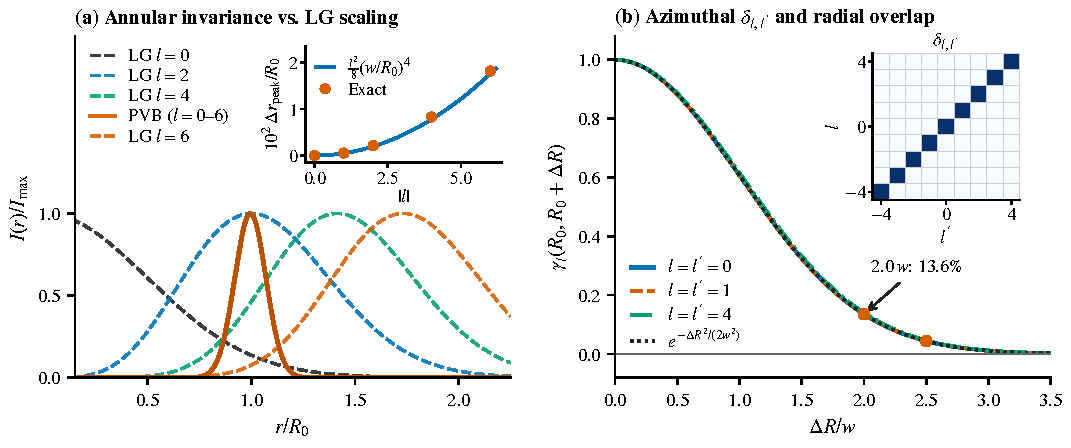
\includegraphics[width=0.94\textwidth]{figures/fig1_pvb_overlap.pdf}
\caption{Physical PVB annular invariance and mutual radial overlap. (a) Peak-normalized radial intensity $I(r)/I_{\max}$ for physical PVBs ($w/R_0 = 0.15$, solid) across $l = 0,2,4,6$ versus $\mathrm{LG}_{0,l}$ ($w_0 = R_0$, dashed); inset compares the exact transcendental differential shift $\Delta r_{\mathrm{peak}}(l)/R_0$ ($w/R_0 = 0.25$, circles) against $(l^2/8)(w/R_0)^4$ [Eq.~\eqref{eq:peak_shift}]. (b) Unit-normalized radial overlap $\gamma_l(R_0, R_0+\Delta R)$ [Eq.~\eqref{eq:gamma_normalized}] at $R_0 = 4w$ for $l = 0,1,4$ versus the $l$-independent Gaussian asymptote $e^{-\Delta R^2/(2w^2)}$ (dotted), marking $13.6\%$ at $\Delta R = 2.0\,w$ and $4.40\%$ at $\Delta R = 2.5\,w$; inset confirms azimuthal Kronecker orthogonality $\delta_{l,l'}$.}
\label{fig:pvb_overlap}
\end{figure*}

\subsection{Optical Fourier Generation and Two-Zone Propagation Regimes}
\label{subsec:generation_bridge}

Physically, $\Phi_{l,R}$ is synthesized as the $2f$ optical Fourier transform of an input Bessel--Gaussian (BG) wavefield~\cite{Vaity2015,Gori1987},
\begin{equation}
E_{\mathrm{BG}}(\rho,\theta) = E_0 J_l(k_r\rho)\exp\!\left(-\frac{\rho^2}{w_g^2}\right) e^{il\theta},
\label{eq:bg_input}
\end{equation}
where $k_r = k_0 (n_{\mathrm{ax}} - 1)\beta$ is the radial conical wavevector, $k_0 = 2\pi/\lambda$ is the free-space wavenumber, $w_g$ is the illuminating Gaussian waist, and $\beta$ is the thin-axicon base (wedge) angle (full apex angle $\pi - 2\beta$). Positioning the BG waist at the front focal plane $d_{\mathrm{in}} = f$ before a spherical lens of focal length $f$ eliminates the quadratic Fresnel phase $\exp[ik_0 r^2(1 - d_{\mathrm{in}}/f)/(2f)]$, yielding Eq.~\eqref{eq:pvb_mode} at the back focal plane ($z = 0$, distance $2f$ from the input waist) with~\cite{Vaity2015}
\begin{equation}
R = \frac{k_r f}{k_0} = (n_{\mathrm{ax}} - 1)\beta f, \qquad w = \frac{2f}{k_0 w_g},
\label{eq:R_w_2f}
\end{equation}
up to the global propagation phase $(-i)^{l+1} e^{2ik_0 f}$ arising from signed $J_l(k_r\rho)$ in Eq.~\eqref{eq:bg_input} [or $(-i)^{\abs{l}+1} e^{2ik_0 f}$ when $J_{\abs{l}}(k_r\rho)$ is imprinted]. Matching the frame prefactor $C_0$ in Eq.~\eqref{eq:C0_norm} fixes the input BG amplitude to
\begin{equation}
E_0 = \frac{1}{w w_g}\sqrt{\frac{2}{\pi}} = \frac{k_0}{f\sqrt{2\pi}},
\label{eq:E0_bridge}
\end{equation}
corresponding to total beam power $P_{\mathrm{in}} = \norm{\Phi_{l,R}}_{L^2}^2 \propto w^{-1}$ in the thin-ring regime $R \gg w$.

\begin{remark}[Pre-focal conical self-healing versus post-focal ring diffraction]
\label{rem:propagation}
One must distinguish the two propagation zones of the BG--PVB relay in Eqs.~\eqref{eq:bg_input}--\eqref{eq:R_w_2f}. Preceding the Fourier lens (or after re-collimating $\Phi_{l,R}$ with a second lens), the input BG beam propagates as a conical wavepacket inclined at $\sin\gamma = k_r/k_0 = R/f$; by right-triangle ray geometry, conical rays clear an on-axis circular obstruction of radius $a_{\mathrm{obs}} \le R$ at shadow vertex $z_{\mathrm{heal}} = a_{\mathrm{obs}}/\tan\gamma \approx a_{\mathrm{obs}}/\sin\gamma = k_0 a_{\mathrm{obs}}/k_r \le f$, within the finite axicon walk-off zone $z_{\max} = w_g/\tan\gamma \approx w_g/\sin\gamma = k_0 w_g/k_r$~\cite{Gori1987}. Past the focal waist ($z > 0$ in free space), by contrast, the conical wavevectors have already focused into the flat-phase ring~\eqref{eq:pvb_mode}; subsequent Fresnel propagation undergoes Bessel--Gauss ring diffraction over the annular Rayleigh range $z_R^{\mathrm{ring}} = k_0 w^2/2$, where radial spreading is governed by $1/w$ and $\abs{l}/R$ and local obstructions heal via azimuthal OAM Poynting-vector circulation~\cite{Reddy2016}. For instance, at $\lambda = 1550\,\mathrm{nm}$ with $f = 100\,\mathrm{mm}$, $w_g = 1.0\,\mathrm{mm}$, and $R = 1.0\,\mathrm{mm}$ ($\sin\gamma = 0.01$, $w = 49.3\,\mu\mathrm{m}$), an obstruction $a_{\mathrm{obs}} = 0.5\,R = 0.5\,\mathrm{mm}$ clears pre-focally at $z_{\mathrm{heal}} \approx 50\,\mathrm{mm} \le f$ within $z_{\max} = w_g/\sin\gamma = 100\,\mathrm{mm}$, whereas the post-focal annular Rayleigh range is $z_R^{\mathrm{ring}} = k_0 w^2/2 = 4.93\,\mathrm{mm}$; the pre-focal ($z_{\mathrm{heal}}$) and post-focal ($z_R^{\mathrm{ring}}$) regimes occupy disjoint axial regions on opposite sides of the Fourier transform lens and do not overlap.
\end{remark}

\section{Continuous Hilbert Frame Formalism}
\label{sec:frame_theory}

\subsection{Azimuthal--Radial Decoupling and Mutual Overlap}
\label{subsec:decoupling}

Because the azimuthal OAM harmonics $\{e^{il\phi}/\sqrt{2\pi}\}_{l\in\mathbb{Z}}$ form an orthonormal basis of $L^2(S^1)$, the transverse Hilbert space decomposes into an orthogonal direct sum of fixed-OAM radial sectors:
\begin{align}
\mathcal{H} = L^2(\mathbb{R}^2) &= \bigoplus_{l\in\mathbb{Z}} \mathcal{H}_l, \nonumber \\
\mathcal{H}_l &= \left\{ f(r)\frac{e^{il\phi}}{\sqrt{2\pi}} : \int_0^\infty \abs{f(r)}^2 r\,dr < \infty \right\}.
\label{eq:sector_decomp}
\end{align}
Consequently, any nonorthogonality of physical PVBs is confined strictly to the continuous radial coordinate $R > 0$ within each fixed-$l$ sector $\mathcal{H}_l$ in Eq.~\eqref{eq:sector_decomp}. Evaluating the $L^2(\mathbb{R}^2)$ inner product between $\Phi_{l,R}$ and $\Phi_{l',R'}$ gives
\begin{align}
\braket{\Phi_{l,R}}{\Phi_{l',R'}} &= C_0^2 \int_0^{2\pi} d\phi\, e^{i(l'-l)\phi} \int_0^\infty r\,dr \nonumber \\
&\quad \times \exp\!\left(-\frac{2r^2 + R^2 + R'^2}{w^2}\right) \nonumber \\
&\quad \times I_{\abs{l}}\!\left(\frac{2Rr}{w^2}\right) I_{\abs{l'}}\!\left(\frac{2R'r}{w^2}\right),
\label{eq:overlap_integral}
\end{align}
whose azimuthal integral yields $2\pi\delta_{l,l'}$ [Fig.~\ref{fig:pvb_overlap}(b) inset]. Setting $l' = l$ in Eq.~\eqref{eq:overlap_integral} and using $I_l = I_{\abs{l}}$ ($\operatorname{Re}(\abs{l}) \ge 0 > -1$), the radial integral closes in exact form via Weber's second exponential integral, formula 6.633.2 of Gradshteyn and Ryzhik~\cite{Gradshteyn2014} [analytically continued through $J_\nu(ix) = i^\nu I_\nu(x)$ for $\operatorname{Re}(p) > 0$ and $\operatorname{Re}(\nu) > -1$],
\begin{equation}
\int_0^\infty x\, e^{-p x^2} I_\nu(a x) I_\nu(b x)\,dx = \frac{1}{2p} e^{\frac{a^2 + b^2}{4p}} I_\nu\!\left(\frac{ab}{2p}\right),
\label{eq:weber_identity}
\end{equation}
with $p = 2/w^2$, $a = 2R/w^2$, and $b = 2R'/w^2$. Substituting $C_0$ from Eq.~\eqref{eq:C0_norm} yields
\begin{equation}
\braket{\Phi_{l,R}}{\Phi_{l',R'}} = \delta_{l,l'}\,\frac{1}{w^2}\exp\!\left(-\frac{R^2 + R'^2}{2w^2}\right) I_{\abs{l}}\!\left(\frac{RR'}{w^2}\right),
\label{eq:overlap_closed}
\end{equation}
confirming strict Kronecker orthogonality across $l$ together with strictly positive normalized radial overlap $\gamma_l(R,R') = \braket{\psi_{l,R}}{\psi_{l,R'}}$,
\begin{equation}
\gamma_l(R,R') = \frac{I_{\abs{l}}(RR'/w^2)}{\sqrt{I_{\abs{l}}(R^2/w^2)\,I_{\abs{l}}(R'^2/w^2)}} \in (0,1),
\label{eq:gamma_normalized}
\end{equation}
for all $R \neq R' > 0$ [Fig.~\ref{fig:pvb_overlap}(b)]. For $RR' \gg w^2$, Hankel expansion of Eq.~\eqref{eq:gamma_normalized} yields $\gamma_l(R,R') \approx \exp[-(R-R')^2/(2w^2)]\{1 + [(4l^2 - 1)/16]w^2(R-R')^2/(R^2 R'^2)\}$, proving that radial cross-talk is topologically universal ($l$-independent) at leading order.

\begin{figure*}[t]
\centering
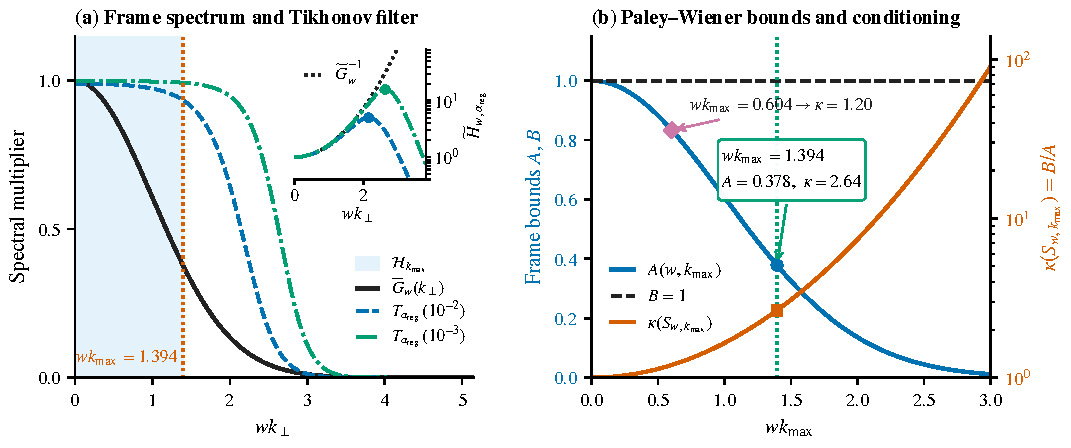
\includegraphics[width=0.94\textwidth]{figures/fig2_frame_regularization.pdf}
\caption{Continuous-frame Fourier spectrum, Tikhonov regularization, and sharp Paley--Wiener bounds. (a) Continuous-frame Fourier multiplier $\widetilde{G}_w(k_\perp)$ and Tikhonov signal transfer $T_{\alpha_{\mathrm{reg}}}(k_\perp)$ ($\alpha_{\mathrm{reg}} = 10^{-2}, 10^{-3}$) with Paley--Wiener passband $\mathcal{H}_{k_{\max}}$ shaded up to $w k_{\max} = 1.394$; inset shows the deconvolution noise gain $\widetilde{H}_{w,\alpha_{\mathrm{reg}}}(k_\perp)$ peaking at $(2\sqrt{\alpha_{\mathrm{reg}}})^{-1}$ [Eq.~\eqref{eq:noise_multiplier}]. (b) Sharp Paley--Wiener bounds $A(w,k_{\max}), B = 1$ and condition number $\kappa(S_{w,k_{\max}}) = B/A$ versus $w k_{\max}$ [Eq.~\eqref{eq:pw_bounds}], highlighting both the weak-attenuation regime ($w k_{\max} = 0.604 \to A = 0.833, \kappa = 1.20$) and the moderate-aperture benchmark ($w k_{\max} = 1.394 \to A = 0.378, \kappa = 2.64$, corresponding to $\mathrm{NA} = 0.20$ at $w/\lambda = 1.11$).}
\label{fig:frame_regularization}
\end{figure*}

\subsection{Continuous Frame Operator, Optimal Bessel Bound, and Convolution Kernel}
\label{subsec:frame_operator}

A family $\{\Phi_\omega\}_{\omega\in\Omega}$ in a separable Hilbert space $\mathcal{H}$ equipped with $\sigma$-finite measure $\mu$ forms a continuous Hilbert frame~\cite{Duffin1952,Daubechies1990,Ali1993,Christensen2016} if $\omega \mapsto \braket{\Phi_\omega}{\psi}$ is measurable and there exist constants $0 < A \le B < \infty$ such that for all $\psi \in \mathcal{H}$,
\begin{equation}
A \norm{\psi}_{\mathcal{H}}^2 \le \int_\Omega \abs{\braket{\Phi_\omega}{\psi}}^2\,d\mu(\omega) \le B \norm{\psi}_{\mathcal{H}}^2.
\label{eq:frame_def}
\end{equation}
If only the upper inequality holds ($B < \infty$), $\{\Phi_\omega\}$ is a continuous Bessel family. With index space $\Omega = \mathbb{Z} \times (0,\infty)$, product measure $d\mu(l,R) = R\,dR$, and analysis operator $(T\psi)(l,R) = \braket{\Phi_{l,R}}{\psi}$, the PVB frame operator $S_w = T^* T : \mathcal{H} \to \mathcal{H}$ is defined by
\begin{equation}
S_w\psi = \sum_{l\in\mathbb{Z}} \int_0^\infty R\,dR\, \braket{\Phi_{l,R}}{\psi}\Phi_{l,R},
\label{eq:frame_op}
\end{equation}
understood in the weak (Pettis) operator sense $\braket{\phi}{S_w\psi} = \sum_{l\in\mathbb{Z}}\int_0^\infty R\,dR\,\braket{\phi}{\Phi_{l,R}}\braket{\Phi_{l,R}}{\psi}$ for all $\phi,\psi \in \mathcal{H}$ (with absolute convergence guaranteed by Lemma~\ref{lem:bessel_upper}). We adopt the non-unitary 2D spatial Fourier transform convention
\begin{align}
\widetilde{\psi}(\mathbf{k}) \equiv \mathcal{F}\{\psi\}(\mathbf{k}) &= \int_{\mathbb{R}^2} \psi(\mathbf{r}) e^{-i\mathbf{k}\cdot\mathbf{r}}\,d^2\mathbf{r}, \nonumber \\
\psi(\mathbf{r}) &= \int_{\mathbb{R}^2} \widetilde{\psi}(\mathbf{k}) e^{i\mathbf{k}\cdot\mathbf{r}}\,\frac{d^2\mathbf{k}}{(2\pi)^2},
\label{eq:ft_convention}
\end{align}
with radial spatial frequency $k_\perp = \abs{\mathbf{k}} = \sqrt{k_x^2 + k_y^2}$ and Plancherel identity $\braket{\phi}{\psi}_{L^2} = (2\pi)^{-2}\braket{\widetilde{\phi}}{\widetilde{\psi}}_{L^2}$.

\begin{lemma}[Continuous Bessel system with optimal upper bound $B=1$]
\label{lem:bessel_upper}
Under the scaling $C_0$ of Eq.~\eqref{eq:C0_norm} and measure \mbox{$d\mu(l,R) = R\,dR$}, the physical PVB family $\{\Phi_{l,R}\}_{l\in\mathbb{Z},\,R>0}$ satisfies for every $\psi \in L^2(\mathbb{R}^2)$
\begin{equation}
\norm{T\psi}_{L^2(\Omega,\mu)}^2 = \int_{\mathbb{R}^2} e^{-w^2 k_\perp^2/2}\abs{\widetilde{\psi}(\mathbf{k})}^2\,\frac{d^2\mathbf{k}}{(2\pi)^2} \le \norm{\psi}_{L^2}^2,
\label{eq:bessel_lemma}
\end{equation}
establishing that $\{\Phi_{l,R}\}$ is a continuous Bessel system on $L^2(\mathbb{R}^2)$ with optimal upper bound $B = 1$.
\end{lemma}
\begin{proof}
Expanding $e^{-i\mathbf{k}\cdot\mathbf{r}}$ via the Jacobi--Anger identity gives the azimuthal integral $\int_0^{2\pi} e^{il\phi - ik_\perp r\cos(\phi-\phi_k)}\,d\phi = 2\pi (-i)^l e^{il\phi_k} J_l(k_\perp r) = 2\pi (-i)^{\abs{l}} e^{il\phi_k} J_{\abs{l}}(k_\perp r)$ for every $l \in \mathbb{Z}$ [using $J_{-n}(z) = (-1)^n J_n(z)$ and $(-i)^{-n} = i^n = (-1)^n(-i)^n$ for integer $n \ge 0$, so both sides agree]. Setting $p = 1/w^2 > 0$, $a = 2R/w^2$, and $\nu = \abs{l} > -1$ in Weber's second exponential integral~\eqref{eq:weber_identity} (formula 6.633.2 of Ref.~\cite{Gradshteyn2014})---valid by analytic continuation in $b \in \mathbb{C}$ for $\operatorname{Re}(p) > 0$ and $\operatorname{Re}(\nu) > -1$, with the limit $b \to -i k_\perp$ taken along the imaginary axis using $I_{\abs{l}}(-i z) = (-i)^{\abs{l}} J_{\abs{l}}(z)$ on both sides (yielding formula 6.633.4 of Ref.~\cite{Gradshteyn2014}, 8th ed.)---gives $\int_0^\infty r\,e^{-r^2/w^2} I_{\abs{l}}(2Rr/w^2) J_{\abs{l}}(k_\perp r)\,dr = (w^2/2)\exp(R^2/w^2 - w^2 k_\perp^2/4) J_{\abs{l}}(R k_\perp)$. Multiplying by $2\pi C_0 e^{-R^2/w^2}$ with $C_0 = w^{-2}\sqrt{2/\pi}$ [Eq.~\eqref{eq:C0_norm}] gives the exact 2D Fourier transform under Eq.~\eqref{eq:ft_convention}:
\begin{equation}
\widetilde{\Phi}_{l,R}(\mathbf{k}) = \sqrt{2\pi}\,(-i)^{\abs{l}} e^{il\phi_k} \exp\!\left(-\frac{w^2 k_\perp^2}{4}\right) J_{\abs{l}}(R k_\perp).
\label{eq:pvb_ft}
\end{equation}
Decomposing $\widetilde{\psi}(k_\perp,\phi_k) = \sum_{l\in\mathbb{Z}} \widetilde{\psi}_l(k_\perp)e^{il\phi_k}$ in polar Fourier coordinates, Plancherel's identity gives $(T\psi)(l,R) = \braket{\Phi_{l,R}}{\psi} = (2\pi)^{-1/2} i^{\abs{l}} \allowbreak \int_0^\infty k_\perp\,dk_\perp\, \allowbreak e^{-w^2 k_\perp^2/4}\widetilde{\psi}_l(k_\perp) J_{\abs{l}}(Rk_\perp) = (2\pi)^{-1/2} i^{\abs{l}}\,\mathrm{H}_{\abs{l}}[e^{-w^2 k_\perp^2/4}\widetilde{\psi}_l](R)$. Because the order-$\abs{l}$ Hankel transform $\mathrm{H}_{\abs{l}}[f](R) \equiv \int_0^\infty f(k_\perp) J_{\abs{l}}(R k_\perp) k_\perp\,dk_\perp$ is unitary from $L^2((0,\infty), k_\perp\,dk_\perp)$ onto $L^2((0,\infty), R\,dR)$, integrating $\abs{(T\psi)(l,R)}^2 R\,dR$ over $R \in (0,\infty)$ and summing over $l \in \mathbb{Z}$ yields
\begin{align*}
\norm{T\psi}_{L^2(\Omega,\mu)}^2 &= \frac{1}{2\pi}\sum_{l\in\mathbb{Z}} \int_0^\infty k_\perp\,dk_\perp\,e^{-w^2 k_\perp^2/2}\abs{\widetilde{\psi}_l(k_\perp)}^2 \\
&= \int_{\mathbb{R}^2} e^{-w^2 k_\perp^2/2}\abs{\widetilde{\psi}(\mathbf{k})}^2\,\frac{d^2\mathbf{k}}{(2\pi)^2}.
\end{align*}
Since $0 < e^{-w^2 k_\perp^2/2} \le 1$ for all $k_\perp \ge 0$, Parseval's identity gives $\norm{T\psi}_{L^2(\Omega,\mu)}^2 \le (2\pi)^{-2}\norm{\widetilde{\psi}}_{L^2}^2 = \norm{\psi}_{L^2}^2$. Optimality of $B = 1$ follows by taking unit-$L^2$-normalized test fields $\widetilde{\psi}_n(\mathbf{k}) = 2\pi(\pi/n^2)^{-1/2}\mathbf{1}_{\{k_\perp \le 1/n\}}(\mathbf{k})$ supported in shrinking balls $B(0,1/n)$; since $e^{-w^2 k_\perp^2/2} \to 1$ uniformly on $B(0,1/n)$ as $n \to \infty$ (and by dominated convergence), $\norm{T\psi_n}_{L^2(\Omega,\mu)}^2/\norm{\psi_n}_{L^2}^2 \to 1$.
\end{proof}

\begin{proposition}[Azimuthal--radial decoupling and Gaussian convolution kernel]
\label{prop:conv_kernel}
For any $w > 0$, the PVB family $\{\Phi_{l,R}\}_{l\in\mathbb{Z},\,R>0}$ obeys Eq.~\eqref{eq:overlap_closed}, and its frame operator~\eqref{eq:frame_op} acts on $L^2(\mathbb{R}^2)$ as the isotropic Gaussian convolution $(S_w\psi)(\mathbf{r}) = (G_w * \psi)(\mathbf{r})$ with kernel $G_w(\mathbf{r}) = (2\pi w^2)^{-1}\exp(-\abs{\mathbf{r}}^2/(2w^2))$, diagonalized in Fourier space as
\begin{equation}
\mathcal{F}\{S_w\psi\}(\mathbf{k}) = \widetilde{G}_w(k_\perp)\widetilde{\psi}(\mathbf{k}), \quad \widetilde{G}_w(k_\perp) = e^{-w^2 k_\perp^2/2}.
\label{eq:fourier_diag}
\end{equation}
Consequently, $S_w$ is positive, bounded ($\norm{S_w} = 1$), and self-adjoint on $L^2(\mathbb{R}^2)$ with purely continuous spectrum $\sigma(S_w) = [0,1]$ given by $\{e^{-w^2 k_\perp^2/2}\}_{k_\perp \ge 0}$ accumulating at $0$ as $k_\perp \to \infty$ (non-compact on unconstrained $L^2(\mathbb{R}^2)$ because its symbol $e^{-w^2 k_\perp^2/2}$ has uncountable essential range $[0,1]$, whereas a compact self-adjoint operator's spectrum is at most countable with $0$ as the only possible accumulation point; it is Hilbert--Schmidt and compact when spatially restricted to any bounded pupil).
\end{proposition}
\begin{proof}
By polarization of Eq.~\eqref{eq:bessel_lemma} in Lemma~\ref{lem:bessel_upper}, for all $\phi,\psi \in L^2(\mathbb{R}^2)$ we have
\begin{align}
\braket{\phi}{S_w\psi} &= \braket{T\phi}{T\psi}_{L^2(\Omega,\mu)} \nonumber \\
&= \int_{\mathbb{R}^2} e^{-w^2 k_\perp^2/2}\widetilde{\phi}^*(\mathbf{k})\widetilde{\psi}(\mathbf{k})\,\frac{d^2\mathbf{k}}{(2\pi)^2} \nonumber \\
&= \int_{\mathbb{R}^2} \widetilde{\phi}^*(\mathbf{k})\!\left[e^{-w^2 k_\perp^2/2}\widetilde{\psi}(\mathbf{k})\right]\frac{d^2\mathbf{k}}{(2\pi)^2} \nonumber \\
&= \braket{\phi}{G_w * \psi},
\label{eq:prop1_polarization}
\end{align}
where we used Plancherel's identity and the convolution theorem $\mathcal{F}\{G_w * \psi\}(\mathbf{k}) = \widetilde{G}_w(k_\perp)\widetilde{\psi}(\mathbf{k})$ with $\mathcal{F}^{-1}\{e^{-w^2 k_\perp^2/2}\}(\mathbf{r}) = (2\pi w^2)^{-1}\exp(-\abs{\mathbf{r}}^2/(2w^2)) = G_w(\mathbf{r})$. Since $\phi \in L^2(\mathbb{R}^2)$ is arbitrary, $S_w\psi = G_w * \psi$, recovering in exact operator form the Gaussian smoothing action noted in Appendix~D of Ref.~\cite{Ferreira2026}. Unitary equivalence via $\mathcal{F}$ to multiplication by the real bounded non-constant radial function $\widetilde{G}_w(k_\perp) \in (0,1]$ establishes positivity, self-adjointness, non-compactness on $\mathbb{R}^2$, and $\sigma(S_w) = \overline{\widetilde{G}_w([0,\infty))} = [0,1]$.
\end{proof}

\subsection{Paley--Wiener Stability Bounds and Physical Obstructions to \texorpdfstring{$w \to 0$}{w -> 0}}
\label{subsec:paley_wiener}

Paraxial optical systems transmit transverse spatial frequencies bounded by a finite aperture cutoff $k_{\max} = k_0 \mathrm{NA}$. Introducing the Paley--Wiener bandlimited Hilbert space
\begin{align}
\mathcal{H}_{k_{\max}} &= \left\{\psi \in L^2(\mathbb{R}^2) : \operatorname{supp}(\widetilde{\psi}) \subseteq \{\abs{\mathbf{k}} \le k_{\max}\}\right\} \nonumber \\
&= \bigoplus_{l\in\mathbb{Z}} \mathcal{H}_{l,k_{\max}},
\label{eq:paley_wiener}
\end{align}
and its orthogonal Fourier-cutoff projector $P_{k_{\max}}\psi = \mathcal{F}^{-1}\{\mathbf{1}_{\{k_\perp \le k_{\max}\}}\widetilde{\psi}\}$, Lemma~\ref{lem:bessel_upper} and Proposition~\ref{prop:conv_kernel} yield our sharp stability theorem.

\begin{theorem}[Paley--Wiener frame stability and projected canonical dual]
\label{thm:pw_bounds}
(i) On unconstrained $L^2(\mathbb{R}^2)$, $\{\Phi_{l,R}\}$ is a continuous Bessel family with optimal upper bound $B = 1$ and vanishing lower bound $A = \inf_{k_\perp \ge 0}\widetilde{G}_w(k_\perp) = 0$; consequently, $S_w^{-1}$ is unbounded on $L^2(\mathbb{R}^2)$ and $S_w^{-1}\Phi_{l,R} \notin L^2(\mathbb{R}^2)$. (ii) Restricted to $\mathcal{H}_{k_{\max}}$ of Eq.~\eqref{eq:paley_wiener} ($0 < k_{\max} < \infty$), the projected family $\{P_{k_{\max}}\Phi_{l,R}\}$ forms a continuous Hilbert frame satisfying Eq.~\eqref{eq:frame_def} with restricted frame operator $S_{w,k_{\max}} = P_{k_{\max}} S_w P_{k_{\max}}\big|_{\mathcal{H}_{k_{\max}}}$, sharp frame bounds
\begin{equation}
A(w,k_{\max}) = \exp\!\left(-\frac{w^2 k_{\max}^2}{2}\right) > 0, \qquad B = 1,
\label{eq:pw_bounds}
\end{equation}
spectral condition number $\kappa(S_{w,k_{\max}}) = B/A = \exp(w^2 k_{\max}^2/2) < \infty$, and bounded canonical dual frame elements $\widetilde{\Phi}_{l,R} = S_{w,k_{\max}}^{-1}P_{k_{\max}}\Phi_{l,R} \in \mathcal{H}_{k_{\max}}$ [Fig.~\ref{fig:frame_regularization}(b)].
\end{theorem}
\begin{proof}
Because $\Phi_{l,R} \in L^2(\mathbb{R}^2)$ (with $\norm{\Phi_{l,R}}_{L^2} < w^{-1}$) and $P_{k_{\max}}$ is an orthogonal projection onto the closed subspace $\mathcal{H}_{k_{\max}}$, we automatically have $P_{k_{\max}}\Phi_{l,R} \in \mathcal{H}_{k_{\max}}$ prior to applying $S_{w,k_{\max}}^{-1}$. For any $\psi \in \mathcal{H}_{k_{\max}}$, self-adjointness of $P_{k_{\max}}$ and $P_{k_{\max}}\psi = \psi$ give $\braket{P_{k_{\max}}\Phi_{l,R}}{\psi} = \braket{\Phi_{l,R}}{\psi}$. By Lemma~\ref{lem:bessel_upper}, $\norm{T\psi}_{L^2(\Omega,\mu)}^2 = \braket{\psi}{S_w\psi} \le \norm{\psi}_{L^2}^2$, giving $B \le 1$, while $\widetilde{G}_w(k_\perp) \ge e^{-w^2 k_{\max}^2/2}$ for all $k_\perp \in [0,k_{\max}]$ gives $\braket{\psi}{S_{w,k_{\max}}\psi} \ge e^{-w^2 k_{\max}^2/2}\norm{\psi}_{L^2}^2$.

To prove sharpness of both constants in Eq.~\eqref{eq:pw_bounds}, define for $\epsilon \in (0,k_{\max})$ the explicit unit-$L^2(\mathbb{R}^2)$-normalized Fourier-annulus test families in $\mathcal{H}_{k_{\max}}$ [accounting for the $(2\pi)^{-2}$ Plancherel prefactor of Eq.~\eqref{eq:ft_convention}]:
\begin{align}
\widetilde{\psi}_\epsilon^{(+)}(\mathbf{k}) &= \frac{2\pi}{\sqrt{\pi\epsilon^2}}\,\mathbf{1}_{\{0 < k_\perp \le \epsilon\}}(\mathbf{k}), \nonumber \\
\widetilde{\psi}_\epsilon^{(-)}(\mathbf{k}) &= \frac{2\pi}{\sqrt{\pi\epsilon(2k_{\max}-\epsilon)}}\,\mathbf{1}_{\{k_{\max}-\epsilon \le k_\perp \le k_{\max}\}}(\mathbf{k}),
\label{eq:fourier_annuli}
\end{align}
where $\pi\epsilon(2k_{\max}-\epsilon) \sim 2\pi k_{\max}\epsilon$ as $\epsilon \to 0^+$ and $\norm{\psi_\epsilon^{(\pm)}}_{L^2}^2 = 1$. Direct radial integration of Eq.~\eqref{eq:bessel_lemma} for Eq.~\eqref{eq:fourier_annuli} yields in closed form
\begin{align}
\braket{\psi_\epsilon^{(+)}}{S_w\psi_\epsilon^{(+)}} &= \frac{2\left(1 - e^{-w^2\epsilon^2/2}\right)}{w^2\epsilon^2} \xrightarrow[\epsilon\to 0^+]{} 1 = B, \nonumber \\
\braket{\psi_\epsilon^{(-)}}{S_w\psi_\epsilon^{(-)}} &= \frac{2\left[e^{-w^2(k_{\max}-\epsilon)^2/2} - e^{-w^2 k_{\max}^2/2}\right]}{w^2\epsilon(2k_{\max}-\epsilon)} \nonumber \\
&\xrightarrow[\epsilon\to 0^+]{} e^{-w^2 k_{\max}^2/2} = A(w,k_{\max}).
\label{eq:sharpness_limits}
\end{align}
Sending $k_{\max} \to \infty$ in Eq.~\eqref{eq:sharpness_limits} proves $\inf_{\norm{\psi}_{L^2}=1}\braket{\psi}{S_w\psi} = 0$ on $L^2(\mathbb{R}^2)$. Finally, because $\widetilde{\Phi}_{l,R}(\mathbf{k})$ in Eq.~\eqref{eq:pvb_ft} has unbounded spatial-frequency support, $\Phi_{l,R} \notin \mathcal{H}_{k_{\max}}$ and $e^{+w^2 k_\perp^2/2}\widetilde{\Phi}_{l,R}(\mathbf{k}) \propto e^{+w^2 k_\perp^2/4} J_{\abs{l}}(Rk_\perp) \notin L^2(\mathbb{R}^2)$, so $S_w^{-1}\Phi_{l,R} \notin L^2(\mathbb{R}^2)$, whereas on $\mathcal{H}_{k_{\max}}$ the restricted multiplier $e^{+w^2 k_\perp^2/2}\mathbf{1}_{\{k_\perp \le k_{\max}\}}$ is bounded by $A^{-1} = e^{w^2 k_{\max}^2/2}$ (and $S_{w,k_{\max}}^{-1/2}$ by $A^{-1/2}$), mapping $P_{k_{\max}}\Phi_{l,R} \in \mathcal{H}_{k_{\max}}$ to $\widetilde{\Phi}_{l,R} \in \mathcal{H}_{k_{\max}}$.
\end{proof}

Notice that $\mathcal{H}_{k_{\max}}$ is a reproducing-kernel Hilbert space (RKHS)~\cite{PaulsenRaghupathi2016} with bandlimited Airy--Bessel reproducing kernel, and that fundamental wave physics forbids taking the singular Dirac limit $w \to 0$: (i) transverse wavevector variance diverges as $\langle k_\perp^2 \rangle \sim w^{-2} \to \infty$, breaking paraxial electrodynamics and converting high-$k_\perp$ tails into evanescent waves above $k_0$; (ii) beam propagation quality degrades as $M^2 \sim R/w \to \infty$; (iii) any finite lens diameter $D$ enforces the diffraction lower bound $w \ge 2\lambda f/(\pi D)$ while fixed optical power $P$ drives peak ring irradiance as $I_{\max} \propto (R w)^{-1}$; and (iv) $\Phi_{l,R}^{\mathrm{ideal}} \notin L^2(\mathbb{R}^2)$ belongs strictly to the distributional dual $\Phi^\times$ of a Gel'fand rigged Hilbert triplet $\Phi \subset L^2(\mathbb{R}^2) \subset \Phi^\times$~\cite{Gelfand1964}. Table~\ref{tab:frame_comparison} synthesizes the structural hierarchy comparing Dirac PVBs, physical PVBs, orthogonal $\mathrm{LG}_{p,l}$ modes, and Glauber coherent states $\ket{\alpha}$~\cite{Klauder1985,Perelomov1986,Gazeau2009}.

\begin{table*}[t]
\caption{Structural comparison of ideal Dirac PVBs, physical finite-width PVBs, Laguerre--Gaussian ($\mathrm{LG}_{p,l}$) eigenmodes, and Glauber coherent states across function space, orthogonality, frame bounds, canonical duals, and radial spatial footprint. Under polar measure $d\mu(l,R) = R\,dR$, $\Phi_{l,R}^{\mathrm{ideal}} = (2\pi)^{-1/2} R^{-1}\delta(r-R)e^{il\phi}$; at the radial endpoint $R = 0$, $\Phi_{l,0} \equiv 0$ ($l \neq 0$) and $\Phi_{0,0}(r) = C_0 e^{-r^2/w^2}$ carries zero $R\,dR$ measure.}
\label{tab:frame_comparison}
\begin{ruledtabular}
\footnotesize
\setlength{\tabcolsep}{3.2pt}
\begin{tabular}{lllll}
Property & Ideal Dirac PVB ($w=0$) & Physical PVB ($w>0$) & $\mathrm{LG}_{p,l}$ Eigenmodes & Coherent States $\ket{\alpha}$ \\
\hline
Function space & Rigged dual $\Phi^\times$ ($\notin L^2$) & $L^2(\mathbb{R}^2)$ (frame on $\mathcal{H}_{k_{\max}}$) & $L^2(\mathbb{R}^2)$ (complete ONB) & Bargmann--Fock $L^2$ \\
Orthogonality & $\delta_{l,l'}\delta(R-R')/R$ & $\delta_{l,l'}$ in $l$; $\gamma_l(R,R') \in (0,1)$ & $\delta_{p,p'}\delta_{l,l'}$ (orthonormal) & $\abs{\braket{\alpha}{\beta}} = e^{-\abs{\alpha-\beta}^2/2}$ \\
Frame bounds & Generalized ONB & $A = e^{-w^2 k_{\max}^2/2},\; B = 1$ ($\mathcal{H}_{k_{\max}}$) & Tight ($A = B = 1$) & Tight ($A = B = 1$, $d^2\alpha/\pi$) \\
Dual / inversion & Self-dual ($\notin L^2$) & $S_w = G_w * \cdot$; Paley--Wiener / Tikhonov & Self-dual ($S = \mathbb{I}$) & Self-dual ($S = \mathbb{I}$) \\
Spatial footprint & Singular ($\langle k_\perp^2\rangle = \infty$) & $l$-invariant ring $R$ [$\Delta r_{\mathrm{peak}} \propto (w/R)^4 R$] & $r_{\mathrm{rms}} = w_0\sqrt{2p+\abs{l}+1}$ & Displaced phase-space packet \\
\end{tabular}
\end{ruledtabular}
\end{table*}

\section{Canonical Dual Regularization, Exact \texorpdfstring{$\mathrm{LG}_{p,l}$}{LG\_\{p,l\}} Expansion, and Discrete Gram Spectrum}
\label{sec:properties}

\subsection{Projected and Tikhonov-Regularized Canonical Dual Frames}
\label{subsec:tikhonov_dual}

When reconstructing a wavefield from noisy frame data, $\psi_{\mathrm{meas}}(\mathbf{r}) = (S_w\psi)(\mathbf{r}) + \varepsilon(\mathbf{r})$ with additive perturbation $\varepsilon(\mathbf{r})$, applying the unregularized inverse multiplier $\widetilde{G}_w^{-1}(k_\perp) = \exp(+w^2 k_\perp^2/2)$ amplifies high-$k_\perp$ noise components $\widetilde{\varepsilon}(\mathbf{k})$ exponentially when $w k_{\max} \gtrsim 1$. To stabilize inversion over $\mathcal{H} \in \{L^2(\mathbb{R}^2), \mathcal{H}_{k_{\max}}\}$, we solve the Tikhonov variational problem with dimensionless regularization weight $\alpha_{\mathrm{reg}} > 0$:
\begin{equation}
\min_{\psi \in \mathcal{H}} \left\{ \norm{S_w\psi - \psi_{\mathrm{meas}}}_{L^2}^2 + \alpha_{\mathrm{reg}}\norm{\psi}_{L^2}^2 \right\}.
\label{eq:tikhonov_opt}
\end{equation}

\begin{proposition}[Tikhonov-regularized dual frame and noise-gain peak]
\label{prop:tikhonov_dual}
For every $\alpha_{\mathrm{reg}} > 0$, the unique minimizer $\hat{\psi}_{\alpha_{\mathrm{reg}}} = S_{w,\alpha_{\mathrm{reg}}}^{-1}\psi_{\mathrm{meas}}$ of Eq.~\eqref{eq:tikhonov_opt} defines the bounded operator
\begin{equation}
S_{w,\alpha_{\mathrm{reg}}}^{-1} = \left(S_w^2 + \alpha_{\mathrm{reg}}\mathbb{I}\right)^{-1} S_w, \qquad \norm{S_{w,\alpha_{\mathrm{reg}}}^{-1}} \le \frac{1}{2\sqrt{\alpha_{\mathrm{reg}}}}.
\label{eq:tikhonov_op_def}
\end{equation}
Because $[S_w, P_{k_{\max}}] = 0$ in the Fourier basis, $S_{w,\alpha_{\mathrm{reg}}}^{-1}$ leaves $\mathcal{H}_{k_{\max}}$ invariant, yielding regularized dual vectors $\widetilde{\Phi}_{l,R}^{(\alpha_{\mathrm{reg}})} = S_{w,\alpha_{\mathrm{reg}}}^{-1}\Phi_{l,R} \in L^2(\mathbb{R}^2)$ (and $S_{w,\alpha_{\mathrm{reg}}}^{-1}P_{k_{\max}}\Phi_{l,R} = P_{k_{\max}}\widetilde{\Phi}_{l,R}^{(\alpha_{\mathrm{reg}})} \in \mathcal{H}_{k_{\max}}$) and spectral deconvolution
\begin{equation}
\mathcal{F}\!\left\{S_{w,\alpha_{\mathrm{reg}}}^{-1}\psi_{\mathrm{meas}}\right\}(\mathbf{k}) = T_{\alpha_{\mathrm{reg}}}(k_\perp)\widetilde{\psi}(\mathbf{k}) + \widetilde{H}_{w,\alpha_{\mathrm{reg}}}(k_\perp)\widetilde{\varepsilon}(\mathbf{k}),
\label{eq:synth_multiplier}
\end{equation}
where $T_{\alpha_{\mathrm{reg}}}(k_\perp) = \widetilde{G}_w^2(k_\perp)/[\widetilde{G}_w^2(k_\perp) + \alpha_{\mathrm{reg}}] < 1$ is the signal shrinkage transfer and
\begin{equation}
\widetilde{H}_{w,\alpha_{\mathrm{reg}}}(k_\perp) = \frac{\widetilde{G}_w(k_\perp)}{\widetilde{G}_w^2(k_\perp) + \alpha_{\mathrm{reg}}} = \frac{e^{-w^2 k_\perp^2/2}}{e^{-w^2 k_\perp^2} + \alpha_{\mathrm{reg}}}.
\label{eq:noise_multiplier}
\end{equation}
For $\alpha_{\mathrm{reg}} \in (0,1)$, $\widetilde{H}_{w,\alpha_{\mathrm{reg}}}(k_\perp)$ attains its global maximum $\widetilde{H}_{\max} = (2\sqrt{\alpha_{\mathrm{reg}}})^{-1}$ at $k_{\mathrm{peak}} = w^{-1}\sqrt{\ln(1/\alpha_{\mathrm{reg}})}$ and decays exponentially as $\alpha_{\mathrm{reg}}^{-1} e^{-w^2 k_\perp^2/2}$ only for $k_\perp \gg k_{\mathrm{peak}}$.
\end{proposition}
\begin{proof}
The Hilbert-space Fr\'echet derivative of Eq.~\eqref{eq:tikhonov_opt} gives $(S_w^2 + \alpha_{\mathrm{reg}}\mathbb{I})\hat{\psi}_{\alpha_{\mathrm{reg}}} = S_w\psi_{\mathrm{meas}}$ (see Appendix~\ref{app:tikhonov_toeplitz} for the full variational and Parseval bias--variance derivation), establishing Eqs.~\eqref{eq:tikhonov_op_def}--\eqref{eq:noise_multiplier}. Since both $S_w$ and $P_{k_{\max}}$ act as radial Fourier multipliers, $[S_w, P_{k_{\max}}] = 0$, so $S_{w,\alpha_{\mathrm{reg}}}^{-1}$ maps $\mathcal{H}_{k_{\max}}$ into itself directly. Writing $\widetilde{H}_{w,\alpha_{\mathrm{reg}}} = (g + \alpha_{\mathrm{reg}}/g)^{-1}$ with $g = \widetilde{G}_w(k_\perp) \in (0,1]$, the arithmetic--geometric mean inequality $g + \alpha_{\mathrm{reg}}/g \ge 2\sqrt{\alpha_{\mathrm{reg}}}$ is saturated uniquely at $g = \sqrt{\alpha_{\mathrm{reg}}}$, i.e., $k_{\mathrm{peak}} = w^{-1}\sqrt{\ln(1/\alpha_{\mathrm{reg}})}$.
\end{proof}

Crucially, contrary to naive intuition that deconvolution roll-off begins near $1/w$, for $\alpha_{\mathrm{reg}} = 10^{-4}$ and $w = 0.5\,\ell_0$ the noise gain rises to $\widetilde{H}_{\max} = 50.0$ at $k_{\mathrm{peak}} = 6.070\,\ell_0^{-1} \gg 1/w = 2.0\,\ell_0^{-1}$ [Fig.~\ref{fig:frame_regularization}(a) inset]. Moreover, because $T_{\alpha_{\mathrm{reg}}}(k_\perp) < 1$ strictly for every $\alpha_{\mathrm{reg}} > 0$, regularized inversion trades controlled shrinkage bias for dramatic variance suppression (quantified in noisy $\mathrm{LG}_{2,1}$ reconstruction in Paper~II~\cite{AyalaPaperII}); zero-bias reconstruction holds exclusively at $\alpha_{\mathrm{reg}} = 0$ on $\mathcal{H}_{k_{\max}}$ via Theorem~\ref{thm:pw_bounds}.

\subsection{Exact Closed-Form Expansion of \texorpdfstring{$\mathrm{LG}_{p,l}$}{LG\_\{p,l\}} Modes (\texorpdfstring{$p \ge 0$}{p >= 0})}
\label{subsec:lg_expansion}

Consider an arbitrary unit-$L^2$-normalized Laguerre--Gaussian eigenmode $\mathrm{LG}_{p,l}$ of waist $w_0$ ($p \in \mathbb{Z}_{\ge 0}$, $l \in \mathbb{Z}$),
\begin{equation}
\psi_{p,l}(r,\phi) = N_{p,l}\left(\frac{\sqrt{2}\,r}{w_0}\right)^{\abs{l}} L_p^{\abs{l}}\!\left(\frac{2r^2}{w_0^2}\right) e^{-r^2/w_0^2 + il\phi},
\label{eq:lg_def}
\end{equation}
with $N_{p,l} = \sqrt{2p!/[\pi(p+\abs{l})!]}/w_0$ and continuous PVB frame analysis coefficients $c_{l,p}(R) = \braket{\Phi_{l,R}}{\psi_{p,l}}$. Extending the $p = 0$ calculation of Ref.~\cite{Ferreira2026} (Appendix~D) to all radial orders $p \ge 0$, we obtain an exact finite algebraic expansion.

\begin{theorem}[Exact closed-form expansion of $\mathrm{LG}_{p,l}$ modes]
\label{thm:c_lp_exact}
For all $p \in \mathbb{Z}_{\ge 0}$, $l \in \mathbb{Z}$, $w > 0$, and $w_0 > 0$, the continuous PVB projection $c_{l,p}(R) = \braket{\Phi_{l,R}}{\psi_{p,l}}$ is given exactly by the $(p+1)$-term finite sum
\begin{equation}
c_{l,p}(R) = \mathcal{A}_{p,l}(R) \sum_{m=0}^p (-1)^m \binom{p+\abs{l}}{p-m} \xi^m L_m^{\abs{l}}(-\zeta_R),
\label{eq:c_lp_exact}
\end{equation}
with dimensionless width parameter and Laguerre argument
\begin{equation}
\xi = \frac{2w^2}{w_0^2 + w^2}, \qquad \zeta_R = \frac{R^2 w_0^2}{w^2(w_0^2 + w^2)},
\label{eq:xi_zeta_defs}
\end{equation}
and envelope prefactor
\begin{align}
\mathcal{A}_{p,l}(R) &= 2^{\frac{\abs{l}}{2}+1}\sqrt{\frac{p!}{(p+\abs{l})!}}\,\frac{R^{\abs{l}} w_0^{\abs{l}+1}}{(w_0^2 + w^2)^{\abs{l}+1}} \nonumber \\
&\quad \times \exp\!\left(-\frac{R^2}{w_0^2 + w^2}\right).
\label{eq:A_prefactor}
\end{align}
These coefficients synthesize the frame-smoothed $\mathrm{LG}_{p,l}$ mode identically via
\begin{equation}
(S_w\psi_{p,l})(\mathbf{r}) = \int_0^\infty R\,dR\, c_{l,p}(R)\,\Phi_{l,R}(\mathbf{r}).
\label{eq:frame_synthesis_lg}
\end{equation}
\end{theorem}

The complete step-by-step derivation---combining the Laguerre generating/polynomial expansion, Gradshteyn--Ryzhik formula 6.631.1~\cite{Gradshteyn2014}, and Kummer's confluent hypergeometric transformation---together with explicit $p = 0$ Weber verification and a 60-point 50-digit quadrature benchmark ($\abs{\Delta c} \le 1.51\times 10^{-15}$, $\abs{\Delta c}/\abs{c} \le 3.64\times 10^{-12} \ll 10^{-6}$) is presented in Appendix~\ref{app:lg_expansion} [Fig.~\ref{fig:lg_washout_gram}(a)]. Computationally, Eq.~\eqref{eq:c_lp_exact} reduces highly oscillatory 2D Bessel--Laguerre overlap integrals to an $\mathcal{O}(p)$ finite algebraic polynomial evaluation via three-term Laguerre recurrence.

\begin{figure*}[t]
\centering
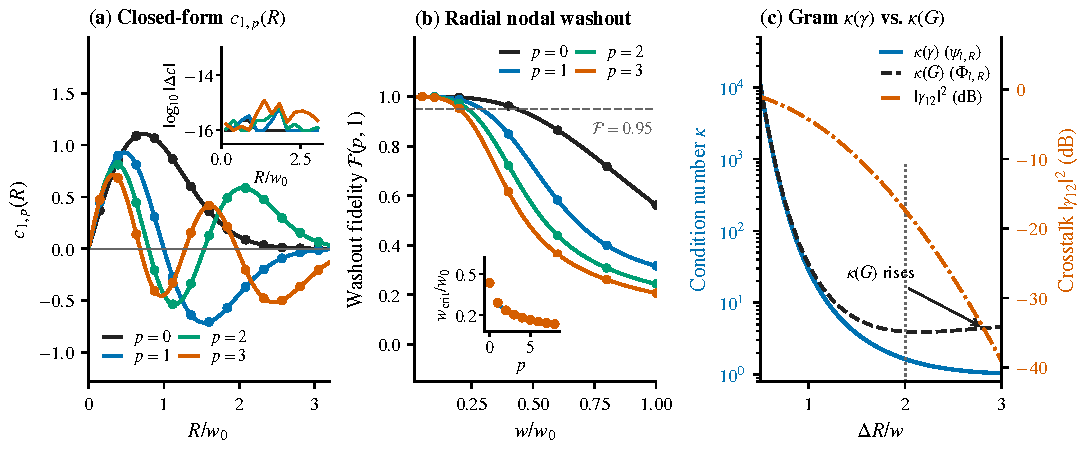
\includegraphics[width=0.98\textwidth]{figures/fig3_lg_washout_gram.pdf}
\caption{Exact Laguerre--Gaussian expansion, radial nodal washout, and discrete radial Gram conditioning. (a) Closed-form coefficients $c_{1,p}(R)$ [Eq.~\eqref{eq:c_lp_exact}, solid] versus adaptive quadrature (circles) for $\mathrm{LG}_{p,1}$ ($p = 0\text{--}3$, $w/w_0 = 0.25$); inset shows $\log_{10}\abs{\Delta c} < -14$. (b) Nodal washout fidelity $\mathcal{F}(p,1,w/w_0)$ [Eq.~\eqref{eq:fidelity_fourier}] with Table~\ref{tab:fidelity} values (dots); inset compares exact $\mathcal{F} = 0.95$ roots $w_{\mathrm{crit}}/w_0$ ($p = 0\text{--}8$) against $0.573/\sqrt{2p+\abs{l}+1}$ ($l = 1$). (c) Monotonic conditioning $\kappa(\gamma)$ of the unit-normalized Gram matrix $[\gamma]_{nm} = \gamma_l(R_n,R_m) = \braket{\psi_{l,R_n}}{\psi_{l,R_m}}$ constructed from normalized states $\{\psi_{l,R_n}\}$ versus diverging $\kappa(G)$ of $[G]_{nm} = \braket{\Phi_{l,R_n}}{\Phi_{l,R_m}}$ constructed from unnormalized frame modes $\{\Phi_{l,R_n}\}$ (left axis), alongside adjacent power crosstalk $\abs{\gamma_{12}}^2$ in dB (right axis) for Table~\ref{tab:gram_matrix}.}
\label{fig:lg_washout_gram}
\end{figure*}

\subsection{Radial Resolution Limits and Nodal Washout}
\label{subsec:nodal_washout}

Because $\psi_{p,l}$ exhibits $p$ concentric interior radial phase-flip nodes~\cite{Allen1992,Siegman1986}, Gaussian convolution by $S_w$ attenuates fine radial structure once $w$ approaches the inter-nodal spacing. Using Eq.~\eqref{eq:fourier_diag} with $u = w_0^2 k_\perp^2/2$, $a = w^2/w_0^2$, and normalized spectral density $\rho_{p,l}(u) = [p!/(p+\abs{l})!]u^{\abs{l}} e^{-u}[L_p^{\abs{l}}(u)]^2$, the uncompensated normalized overlap fidelity $\mathcal{F}(p,l,w/w_0) \equiv \abs{\braket{\psi_{p,l}}{S_w\psi_{p,l}}}^2 / (\norm{\psi_{p,l}}_{L^2}^2 \norm{S_w\psi_{p,l}}_{L^2}^2)$ reduces to
\begin{equation}
\mathcal{F}(p,l,w/w_0) = \frac{\left(\int_0^\infty e^{-au}\,\rho_{p,l}(u)\,du\right)^2}{\int_0^\infty e^{-2au}\,\rho_{p,l}(u)\,du}.
\label{eq:fidelity_fourier}
\end{equation}
Table~\ref{tab:fidelity} reports exact values of Eq.~\eqref{eq:fidelity_fourier} at $l = 1$; notably, at $w/w_0 = 1.00$ they coincide with the exact rational fractions $9/16$, $81/256$, $18225/74752$, and $8037225/38862848$ for $p = 0,1,2,3$.

\begin{table}[t]
\caption{Exact radial reconstruction fidelity $\mathcal{F}(p, l=1, w/w_0)$ of $\mathrm{LG}_{p,1}$ modes under the PVB frame operator $S_w$ across relative ring half-widths $w/w_0$. At $w/w_0 = 1.00$, entries match the exact rationals $9/16$, $81/256$, $18225/74752$, and $8037225/38862848$.}
\label{tab:fidelity}
\begin{ruledtabular}
\setlength{\tabcolsep}{3.5pt}
\begin{tabular}{ccccc}
$w / w_0$ & $\mathcal{F}(p=0)$ & $\mathcal{F}(p=1)$ & $\mathcal{F}(p=2)$ & $\mathcal{F}(p=3)$ \\
\hline
0.05 & 0.99999 & 0.99995 & 0.99989 & 0.99980 \\
0.10 & 0.99980 & 0.99921 & 0.99822 & 0.99683 \\
0.20 & 0.99704 & 0.98782 & 0.97282 & 0.95276 \\
0.40 & 0.96231 & 0.84935 & 0.72301 & 0.61610 \\
0.60 & 0.86477 & 0.58216 & 0.43953 & 0.36419 \\
0.80 & 0.71861 & 0.39960 & 0.30831 & 0.26129 \\
1.00 & 0.56250 & 0.31641 & 0.24381 & 0.20681 \\
\end{tabular}
\end{ruledtabular}
\end{table}

To formalize radial resolution under a single unified benchmark, we define the critical half-width $w_{\mathrm{crit}}(p,l)$ by the $95\%$ overlap-fidelity criterion $\mathcal{F}(p,l,w_{\mathrm{crit}}/w_0) = 0.95$, while distinguishing two physical regimes: (i) for $p = 0$ (nodeless annular modes), $\mathcal{F} < 0.95$ marks envelope-broadening washout (for $l = 1$, $\mathcal{F}$ drops further below $0.50$ only at $w/w_0 = 1.1247$); whereas (ii) for $p \ge 1$, $\mathcal{F} \ge 0.95$ enforces survival of all $p$ interior radial phase-flip nodes without destructive inter-ring smoothing.

\begin{corollary}[Generalized radial Rayleigh criterion]
\label{cor:rayleigh_radial}
Enforcing $\mathcal{F}(p,l,w/w_0) \ge 0.95$ requires: (i) for nodeless $p = 0$ modes, with $q_l \equiv 0.95^{1/(\abs{l}+1)}$, the exact algebraic threshold
\begin{equation}
w \le w_{\mathrm{crit}}(0,l) = w_0 \left[\left(1 - \sqrt{1 - q_l}\right)^{-1} - 1\right]^{1/2},
\label{eq:rayleigh_p0}
\end{equation}
yielding $0.5367\,w_0$ ($l = 0$), $0.4350\,w_0$ ($l = 1$), and $0.3869\,w_0$ ($l = 2$); and (ii) for multi-ring $p \ge 1$ modes, the generalized nodal Rayleigh limit
\begin{equation}
w \lesssim w_{\mathrm{crit}}(p,l) \approx \frac{0.573\,w_0}{\sqrt{2p + \abs{l} + 1}} \qquad (p \ge 1),
\label{eq:rayleigh_radial}
\end{equation}
whose prefactor $0.573$ matches the exact $l = 1$ root within $1.3\%$ at $p = 1$ and within $0.3\%$ for all $p \ge 3$, exhibits only mild $\mathcal{O}(\abs{l}/p)$ centrifugal shifts at small $p/\abs{l}$ ($w_{\mathrm{crit}}\sqrt{2p+\abs{l}+1}/w_0 = 0.5720, 0.5744, 0.5795, 0.5930$ for $\abs{l} = 0,1,2,4$ at $p = 3$), and converges for every fixed $l$ as $p \gg \abs{l}$ to the strictly $(p,l)$-independent arcsine-law asymptote $I_0(c)^2/I_0(2c) = 0.95 \implies \sqrt{c} = 0.5724$ (slightly above the second-cumulant estimate $0.10^{1/4} = 0.5623$).
\end{corollary}
\begin{proof}
At $p = 0$, Eq.~\eqref{eq:fidelity_fourier} evaluates to $\mathcal{F}(0,l,w/w_0) = [(1+2a)/(1+a)^2]^{\abs{l}+1} = [1 - a^2/(1+a)^2]^{\abs{l}+1}$; equating to $0.95$ gives $a/(1+a) = \sqrt{1 - q_l}$ and hence Eq.~\eqref{eq:rayleigh_p0}. For $p \ge 1$, the exact spectral variance $\operatorname{Var}_{\rho_{p,l}}(u) = 2p^2 + 2p\abs{l} + 2p + \abs{l} + 1 \approx \frac{1}{2}(2p+\abs{l}+1)^2$ dictates the $(2p+\abs{l}+1)^{-1/2}$ scaling in Eq.~\eqref{eq:rayleigh_radial}. For $p \gg \abs{l}$, the oscillatory envelope of $\rho_{p,l}(u)$ on $u \in (0, 2(2p+\abs{l}+1))$ approaches the $l$-independent WKB arcsine density $[\pi\sqrt{u(4N_p-u)}]^{-1}$ with $2N_p = 2p+\abs{l}+1$, whose Laplace transform $e^{-2N_p a}I_0(2N_p a)$ reduces Eq.~\eqref{eq:fidelity_fourier} to $I_0(c)^2/I_0(2c)$ with $c = (2p+\abs{l}+1)a$; numerical root-finding at $l = 1$ yields $w_{\mathrm{crit}}\sqrt{2p+\abs{l}+1}/w_0 = 0.5806\,(p=1), 0.5759\,(p=2), 0.5744\,(p=3), 0.5727\,(p=10)$, converging monotonically to $0.5724$ [Fig.~\ref{fig:lg_washout_gram}(b) inset].
\end{proof}

\subsection{Discrete Radial Sampling and Unit-Normalized Gram Spectrum}
\label{subsec:gram_sampling}

Discretizing $N$ concentric ring radii $R_n = R_{\min} + (n-1)\Delta R$ ($n = 1,\dots,N$) at fixed $l$ defines two distinct finite matrices: the unnormalized frame Gram matrix $[G]_{nm} = G_{nm} = \braket{\Phi_{l,R_n}}{\Phi_{l,R_m}}$ built from $\{\Phi_{l,R_n}\}$ via Eq.~\eqref{eq:overlap_closed}, and the unit-normalized state Gram matrix $[\gamma]_{nm} = \gamma_l(R_n,R_m)$ built from the unit-$L^2$-normalized states $\{\psi_{l,R_n}\}$ via Eq.~\eqref{eq:gamma_normalized}:
\begin{equation}
[\gamma]_{nm} = \gamma_{nm} = \frac{G_{nm}}{\sqrt{G_{nn}\,G_{mm}}} = \braket{\psi_{l,R_n}}{\psi_{l,R_m}}.
\label{eq:gram_normalized}
\end{equation}
Because $G_{nn} \approx (2\pi R_n^2 w^2)^{-1/2}$ decays as $R_n^{-1}$, the unnormalized condition number $\kappa(G) = \lambda_{\max}(G)/\lambda_{\min}(G)$ grows spuriously with $N$ even when rings are well separated (at $N = 120$ and $\Delta R = 2.0\,w$, $\kappa(G) = 80.02$ whereas $\kappa(\gamma) = 1.741$). Stability of the finite radial subspace $\operatorname{span}\{\psi_{l,R_n}\}_{n=1}^N$ and its canonical biorthogonal dual $\{\tilde{\psi}_{l,n} = \sum_{m=1}^N (\gamma^{-1})_{mn}\psi_{l,R_m}\}$ is governed strictly by $[\gamma]_{nm}$ in Eq.~\eqref{eq:gram_normalized}. Specifically, substituting $R_n - R_m = (n-m)\Delta R$ into the Hankel expansion of Eq.~\eqref{eq:gamma_normalized} in the annular regime $R_{\min} \gg w, \abs{l}w/2$ gives $[\gamma]_{nm} = \exp[-(n-m)^2\Delta R^2/(2w^2)][1 + \mathcal{O}((4l^2-1)w^2(n-m)^2\Delta R^2/R_{\min}^4)]$, which depends at leading order solely on the index difference $n - m$. In particular, adjacent rings ($m = n+1$) satisfy
\begin{equation}
\gamma_{n,n+1} \approx \exp\!\left(-\frac{\Delta R^2}{2w^2}\right),
\label{eq:crosstalk_asymptotic}
\end{equation}
with squared power overlap $\abs{\gamma_{n,n+1}}^2 \approx \exp(-\Delta R^2/w^2)$, whereas near the origin Eq.~\eqref{eq:crosstalk_asymptotic} breaks down (at $R_{\min} = 0.2\,w, l = 1, \Delta R = 2.0\,w$, exact $\gamma_{12} = 34.76\%$ versus $e^{-2} = 13.53\%$).

\begin{proposition}[Discrete radial sampling and Jacobi-theta Toeplitz bound]
\label{prop:channel_capacity}
In the annular regime $R_{\min} \gg w, \abs{l}w/2$, the unit-normalized Gram matrix $[\gamma]_{nm}$ converges entrywise to the symmetric Gaussian Toeplitz matrix $T_{n-m} = q^{(n-m)^2}$ with $q = e^{-\Delta R^2/(2w^2)}$, whose condition number is bounded uniformly for all $N \in \mathbb{N}$ by the Jacobi-theta ratio $\kappa(T_\infty) = \vartheta_3(0,q)/\vartheta_4(0,q)$ (Appendix~\ref{app:tikhonov_toeplitz}). Enforcing $\Delta R \ge 2.0\,w$ guarantees $\kappa(\gamma) = 1.645$ for $N = 6$ ($\le 1.7416$ for all $N$ in the asymptotic Toeplitz limit), adjacent overlap $\le 13.6\%$ (power isolation $\ge 17.36\,\mathrm{dB}$, from $-10\log_{10}\abs{\gamma_{12}}^2$ at $\abs{\gamma_{12}} = 0.1355$), and normalized dual-frame trace invariants $\operatorname{Tr}(\gamma^{-1})/N = 1.032$ ($0.14\,\mathrm{dB}$) and $\operatorname{Tr}(\gamma^{-2})/N = 1.099$ ($0.41\,\mathrm{dB}$) for $N = 6$ ($< 0.50\,\mathrm{dB}$ for all $N$). Over radial span $\mathcal{W} = R_{\max} - R_{\min}$, the maximum well-conditioned ring count at fixed $l$ is
\begin{equation}
N_{\max} \approx \left\lfloor \frac{\mathcal{W}}{2w} \right\rfloor + 1.
\label{eq:channel_capacity}
\end{equation}
\end{proposition}

Table~\ref{tab:gram_matrix}, Eq.~\eqref{eq:channel_capacity}, and Fig.~\ref{fig:lg_washout_gram}(c) confirm monotonic stabilization of $\kappa(\gamma)$, reaching quasi-orthogonal isolation ($27.13\,\mathrm{dB}$ power isolation, $\kappa(\gamma) = 1.172$) at $\Delta R = 2.5\,w$.

\begin{table*}[t]
\caption{Unit-normalized Gram conditioning $\kappa(\gamma)$ (built from $\{\psi_{l,R_n}\}$), unnormalized $\kappa(G)$ (built from $\{\Phi_{l,R_n}\}$), adjacent overlap/isolation, and canonical dual-frame trace invariants for $N = 6$ concentric radial PVB modes ($w = 0.5\,\ell_0$, $l = 1$, $R_{\min} = 2.0\,\ell_0$, in arbitrary length units $\ell_0$).}
\label{tab:gram_matrix}
\begin{ruledtabular}
\footnotesize
\setlength{\tabcolsep}{2.5pt}
\begin{tabular}{ccccccccc}
$\Delta R / w$ & $\Delta R\,(\ell_0)$ & $\abs{\gamma_{12}}$ & $\abs{\gamma_{12}}^2$ (Iso.) & $\kappa(\gamma)$ & $\kappa(G)$ & $\operatorname{Tr}(\gamma^{-1})/N$ & $\operatorname{Tr}(\gamma^{-2})/N$ & Regime \\
\hline
0.50 & 0.250 & $88.26\%$ & $77.91\%$ ($1.08$~dB) & $1.086\times 10^4$ & $1.123\times 10^4$ & $502.0$ ($27.01$~dB) & $1.364\times 10^6$ ($61.35$~dB) & Ill-conditioned \\
1.00 & 0.500 & $60.68\%$ & $36.83\%$ ($4.34$~dB) & $28.80$ & $34.30$ & $3.418$ ($5.34$~dB) & $30.14$ ($14.79$~dB) & Ill-conditioned \\
1.50 & 0.750 & $32.50\%$ & $10.56\%$ ($9.76$~dB) & $3.723$ & $5.960$ & $1.237$ ($0.92$~dB) & $1.890$ ($2.76$~dB) & Transition \\
2.00 & 1.000 & $13.55\%$ & $1.84\%$ ($17.36$~dB) & $1.645$ & $3.959$ & $1.032$ ($0.14$~dB) & $1.099$ ($0.41$~dB) & Optimal \\
2.50 & 1.250 & $4.40\%$ & $0.194\%$ ($27.13$~dB) & $1.172$ & $4.096$ & $1.003$ ($0.01$~dB) & $1.010$ ($0.04$~dB) & Quasi-orthogonal \\
3.00 & 1.500 & $1.11\%$ & $0.012\%$ ($39.07$~dB) & $1.041$ & $4.646$ & $1.000$ ($0.00$~dB) & $1.001$ ($0.00$~dB) & Quasi-orthogonal \\
\end{tabular}
\end{ruledtabular}
\end{table*}

\section{Conclusions}
\label{sec:conclusions}

We have established a complete operator-theoretic formulation of physical finite-width PVBs as continuous Hilbert frames. While azimuthal OAM sectors decouple into strictly orthogonal subspaces ($\mathcal{H} = \bigoplus_{l\in\mathbb{Z}}\mathcal{H}_l$), finite ring half-width $w > 0$ induces a positive self-adjoint isotropic Gaussian convolution frame operator $S_w = G_w * \cdot$ with purely continuous spectrum $[0,1]$, optimal Bessel upper bound $B = 1$, vanishing global lower bound $A = 0$ on unconstrained $L^2(\mathbb{R}^2)$, and sharp Paley--Wiener stability bounds $A = \exp(-w^2 k_{\max}^2/2)$ and $B = 1$ on $\mathcal{H}_{k_{\max}}$ (Lemma~\ref{lem:bessel_upper}, Proposition~\ref{prop:conv_kernel}, and Theorem~\ref{thm:pw_bounds}). Furthermore, radial cross-talk is topologically universal ($l$-independent) at leading order. Building on this structure, we constructed the Tikhonov-regularized canonical dual frame and proved its deconvolution noise-gain peak $(2\sqrt{\alpha_{\mathrm{reg}}})^{-1}$ at $k_{\mathrm{peak}} = w^{-1}\sqrt{\ln(1/\alpha_{\mathrm{reg}})}$ (Proposition~\ref{prop:tikhonov_dual}), proved the exact $(p+1)$-term closed-form expansion $c_{l,p}(R)$ for all $\mathrm{LG}_{p,l}$ modes ($p \ge 0$, Theorem~\ref{thm:c_lp_exact}), established both the exact $p = 0$ threshold and the generalized nodal Rayleigh limit $w_{\mathrm{crit}} \approx 0.573\,w_0/\sqrt{2p+\abs{l}+1}$ ($p \ge 1$, Corollary~\ref{cor:rayleigh_radial}), and proved monotonic unit-normalized Gram conditioning bounded by the Jacobi-theta Toeplitz limit ($\kappa(\gamma) = 1.645$ at $\Delta R = 2.0\,w$, Proposition~\ref{prop:channel_capacity}). In Paper~II~\cite{AyalaPaperII}, these exact operator results are applied to noisy modal reconstruction, ring-core fiber multiplexing, atmospheric turbulence filtering, multi-plane radial-qudit quantum tomography, and entangled aperture invariance.

\begin{acknowledgments}
AI disclosure: Portions of this work were developed with the assistance of Gemini~4~Carbon (Google DeepMind) operating within the Antigravity IDE (accessed November 2026). The AI was used for symbolic calculus, asymptotic expansions, numerical verification scripting, and \LaTeX{} typesetting. All hypotheses, domain specifications, proofs, and physical interpretations were conceived and audited by the human author, Sebasti\'an Ayala, who takes full responsibility for the integrity and accuracy of the manuscript in accordance with American Physical Society editorial policies.
\end{acknowledgments}

\section*{Data Availability}
{\sloppy All analytical verification scripts, first-principles numerical routines (\texttt{pvb\_\allowbreak physics.py}, \texttt{verify\_\allowbreak analytical\_\allowbreak tables.py}, and \texttt{generate\_\allowbreak figures.py}), and 50-digit benchmark datasets (\texttt{theorem2\_\allowbreak table\_\allowbreak 60.json} and \texttt{verified\_\allowbreak metrics.json}) supporting the findings of this study are openly available at \href{https://github.com/ayalaphysds/Paper-propiedades-base-sobre-completa-PVB}{\texttt{github.com/\allowbreak ayalaphysds/\allowbreak Paper-\allowbreak propiedades-\allowbreak base-\allowbreak sobre-\allowbreak completa-\allowbreak PVB}} (archived at Zenodo, DOI:~\href{https://doi.org/10.5281/zenodo.24426770}{\texttt{10.5281/\allowbreak zenodo.\allowbreak 24426770}}; MIT License, including a \texttt{README} with one-command reproduction instructions for Figs.~1--3 and Tables~I--IV) and in the accompanying journal/arXiv ancillary code archive.\par}

\appendix

\section{Derivation and Quadrature Verification of the Closed-Form \texorpdfstring{$\mathrm{LG}_{p,l}$}{LG\_\{p,l\}} Expansion}
\label{app:lg_expansion}

Evaluating $c_{l,p}(R) = \braket{\Phi_{l,R}}{\psi_{p,l}}$ from Eqs.~\eqref{eq:pvb_mode} and~\eqref{eq:lg_def} and integrating over $\phi \in [0,2\pi)$ gives
\begin{align}
c_{l,p}(R) &= 2\pi C_0 N_{p,l} e^{-R^2/w^2} \int_0^\infty r\,dr\, e^{-a_0 r^2} I_{\abs{l}}(b_R r) \nonumber \\
&\quad \times \left(\frac{\sqrt{2}\,r}{w_0}\right)^{\abs{l}} L_p^{\abs{l}}\!\left(\frac{2r^2}{w_0^2}\right),
\label{eq:app_c_int}
\end{align}
where $a_0 = 1/w^2 + 1/w_0^2 = (w_0^2+w^2)/(w^2 w_0^2)$, $b_R = 2R/w^2$, $N_{p,l} = \sqrt{2p!/[\pi(p+\abs{l})!]}/w_0$, and $I_l(b_R r) = I_{\abs{l}}(b_R r)$ for $l \in \mathbb{Z}$.

Before treating general $p \ge 0$, we verify the fundamental $p = 0$ limit directly via Weber's first exponential integral. For $p = 0$ and $l = 0$, $L_0^0 \equiv 1$ and $N_{0,0} = w_0^{-1}\sqrt{2/\pi}$, so Eq.~\eqref{eq:app_c_int} reduces to
\begin{align}
c_{0,0}(R) &= \frac{4}{w^2 w_0} e^{-R^2/w^2} \int_0^\infty r\,e^{-a_0 r^2} I_0(b_R r)\,dr \nonumber \\
&= \frac{4}{w^2 w_0} e^{-R^2/w^2} \frac{1}{2a_0} \exp\!\left(\frac{b_R^2}{4a_0}\right) \nonumber \\
&= \frac{2w_0}{w_0^2 + w^2} \exp\!\left(-\frac{R^2}{w_0^2 + w^2}\right) = \mathcal{A}_{0,0}(R),
\label{eq:app_p0_l0_check}
\end{align}
since $-R^2/w^2 + b_R^2/(4a_0) = -R^2/(w_0^2 + w^2)$. More generally, at $p = 0$ and any $l \in \mathbb{Z}$, $L_0^{\abs{l}} \equiv 1$ and Gradshteyn--Ryzhik formula 6.631.4~\cite{Gradshteyn2014} gives $\int_0^\infty r^{\abs{l}+1} e^{-a_0 r^2} I_{\abs{l}}(b_R r)\,dr = b_R^{\abs{l}} (2 a_0)^{-\abs{l}-1} e^{b_R^2/(4a_0)}$, reproducing $c_{l,0}(R) = \mathcal{A}_{0,l}(R)$ in exact agreement with Appendix~D of Ref.~\cite{Ferreira2026} up to the unit-norm factor $\norm{\Phi_{l,R}}_{L^2}^{-1}$ (and verified against 50-digit quadrature in rows 1--3 and 7--9 of Table~\ref{tab:c_lp_verification}).

For arbitrary $p \ge 0$, using the associated Laguerre generating function $(1-t)^{-\abs{l}-1}\allowbreak \exp[-2r^2 t/(w_0^2(1-t))] = \sum_{p=0}^\infty t^p L_p^{\abs{l}}(2r^2/w_0^2)$ yields the finite polynomial expansion $L_p^{\abs{l}}(2r^2/w_0^2) = \sum_{m=0}^p (-1)^m \allowbreak \binom{p+\abs{l}}{p-m} \allowbreak (m!)^{-1} \allowbreak (2/w_0^2)^m r^{2m}$, separating Eq.~\eqref{eq:app_c_int} into $(p+1)$ radial integrals:
\begin{align}
\mathcal{J}_{p,l} &= \left(\frac{\sqrt{2}}{w_0}\right)^{\abs{l}} \sum_{m=0}^p \frac{(-1)^m}{m!}\binom{p+\abs{l}}{p-m}\left(\frac{2}{w_0^2}\right)^m \nonumber \\
&\quad \times \int_0^\infty r^{\abs{l}+2m+1} e^{-a_0 r^2} I_{\abs{l}}(b_R r)\,dr.
\label{eq:app_J_sum}
\end{align}
Each integral in Eq.~\eqref{eq:app_J_sum} closes via formula 6.631.1 of Gradshteyn and Ryzhik~\cite{Gradshteyn2014}, analytically continued via $J_\nu(i b_R r) = i^\nu I_\nu(b_R r)$ for $\operatorname{Re}(a_0) > 0$ and $\operatorname{Re}(\mu+\nu) > 0$:
\begin{align*}
\int_0^\infty r^{\mu-1} e^{-a_0 r^2} I_\nu(b_R r)\,dr &= \frac{b_R^\nu\,\Gamma\!\left(\frac{\mu+\nu}{2}\right)}{2^{\nu+1} a_0^{(\mu+\nu)/2}\Gamma(\nu+1)} \\
&\quad \times {_1F_1}\!\left(\frac{\mu+\nu}{2}; \nu+1; \frac{b_R^2}{4a_0}\right).
\end{align*}
Setting $\nu = \abs{l} \ge 0$ and $\mu = \abs{l} + 2m + 2$ gives $(\mu+\nu)/2 = \abs{l} + m + 1$, yielding
\begin{align}
&\int_0^\infty r^{\abs{l}+2m+1} e^{-a_0 r^2} I_{\abs{l}}(b_R r)\,dr \nonumber \\
&\quad = \frac{b_R^{\abs{l}}(\abs{l}+m)!}{2^{\abs{l}+1} a_0^{\abs{l}+m+1}\abs{l}!}\,{_1F_1}\!\left(\abs{l}+m+1; \abs{l}+1; \zeta_R\right),
\label{eq:app_hypergeom}
\end{align}
where $\zeta_R = b_R^2/(4a_0) = R^2 w_0^2/[w^2(w_0^2+w^2)]$. Applying Kummer's first transformation ${_1F_1}(a;b;\zeta_R) = e^{\zeta_R}\,{_1F_1}(b-a;b;-\zeta_R)$ to Eq.~\eqref{eq:app_hypergeom} sets $b - a = -m$, terminating the hypergeometric series as an associated Laguerre polynomial of degree $m$:
\begin{equation}
{_1F_1}\!\left(-m; \abs{l}+1; -\zeta_R\right) = \frac{m!\,\abs{l}!}{(\abs{l}+m)!}\,L_m^{\abs{l}}(-\zeta_R).
\label{eq:app_kummer_laguerre}
\end{equation}
Canceling the factorials $m!$, $\abs{l}!$, and $(\abs{l}+m)!$ between Eqs.~\eqref{eq:app_J_sum}--\eqref{eq:app_kummer_laguerre}, identifying $[2/(a_0 w_0^2)]^m = \xi^m$, and collecting $2\pi C_0 N_{p,l} b_R^{\abs{l}} 2^{-(\abs{l}+1)} a_0^{-(\abs{l}+1)} (\sqrt{2}/w_0)^{\abs{l}} e^{-R^2/w^2 + \zeta_R} = \mathcal{A}_{p,l}(R)$ proves Eqs.~\eqref{eq:c_lp_exact}--\eqref{eq:A_prefactor} of Theorem~\ref{thm:c_lp_exact}. Table~\ref{tab:c_lp_verification} benchmarks Eq.~\eqref{eq:c_lp_exact} against 50-digit numerical quadrature across 60 parameter combinations, confirming $\abs{\Delta c}/\abs{c} \le 3.64\times 10^{-12} \ll 10^{-6}$ throughout.

\begin{table*}[t]
\caption{Numerical verification of the closed-form $\mathrm{LG}_{p,l}$ frame expansion $c_{l,p}(R)$ [Eq.~\eqref{eq:c_lp_exact}] against arbitrary-precision radial quadrature of Eq.~\eqref{eq:app_c_int} across $(p,l) \in \{(0,0),(1,0),(0,1),(2,1),(3,2)\}$, $w/w_0 \in \{0.25,0.50,1.00\}$, and $R/w_0 \in \{0.5,1.0,1.5,2.0\}$ ($w_0 = 1$, 60 total entries). Closed-form and quadrature values agree identically to all six displayed significant digits; the rightmost column reports the maximum IEEE-754 relative discrepancy $\max_R \abs{c_{\mathrm{exact}} - c_{\mathrm{quad}}}/\abs{c_{\mathrm{quad}}}$ across the four radii in each row.}
\label{tab:c_lp_verification}
\begin{ruledtabular}
\footnotesize
\begin{tabular}{ccccccc}
Mode $(p,l)$ & $w/w_0$ & $c_{l,p}(0.5\,w_0)$ & $c_{l,p}(1.0\,w_0)$ & $c_{l,p}(1.5\,w_0)$ & $c_{l,p}(2.0\,w_0)$ & $\max_R \abs{\Delta c}/\abs{c}$ \\
\hline
$(0,0)$ & $0.25$ & $+1.487696$ & $+0.734435$ & $+0.226474$ & $+0.043622$ & $1.23\times 10^{-16}$ \\
$(0,0)$ & $0.50$ & $+1.309969$ & $+0.718926$ & $+0.264478$ & $+0.065220$ & $1.70\times 10^{-16}$ \\
$(0,0)$ & $1.00$ & $+0.882497$ & $+0.606531$ & $+0.324652$ & $+0.135335$ & $< 1.0\times 10^{-16}$ \\
\hline
$(1,0)$ & $0.25$ & $+0.653762$ & $-0.653113$ & $-0.702932$ & $-0.270640$ & $1.70\times 10^{-16}$ \\
$(1,0)$ & $0.50$ & $+0.366791$ & $-0.488870$ & $-0.603010$ & $-0.294792$ & $2.27\times 10^{-16}$ \\
$(1,0)$ & $1.00$ & $-0.110312$ & $-0.303265$ & $-0.365234$ & $-0.270671$ & $< 1.0\times 10^{-16}$ \\
\hline
$(0,1)$ & $0.25$ & $+0.990080$ & $+0.977551$ & $+0.452164$ & $+0.116125$ & $2.39\times 10^{-16}$ \\
$(0,1)$ & $0.50$ & $+0.741030$ & $+0.813372$ & $+0.448834$ & $+0.147575$ & $1.50\times 10^{-16}$ \\
$(0,1)$ & $1.00$ & $+0.312010$ & $+0.428882$ & $+0.344346$ & $+0.191393$ & $1.78\times 10^{-16}$ \\
\hline
$(2,1)$ & $0.25$ & $+0.721001$ & $-0.442836$ & $-0.070805$ & $+0.582387$ & $4.12\times 10^{-15}$ \\
$(2,1)$ & $0.50$ & $+0.237534$ & $-0.190094$ & $+0.011195$ & $+0.423558$ & $2.77\times 10^{-14}$ \\
$(2,1)$ & $1.00$ & $+0.001407$ & $+0.030952$ & $+0.125808$ & $+0.221002$ & $3.08\times 10^{-16}$ \\
\hline
$(3,2)$ & $0.25$ & $+0.565705$ & $-0.269604$ & $+0.066491$ & $+0.218546$ & $2.28\times 10^{-14}$ \\
$(3,2)$ & $0.50$ & $+0.108369$ & $-0.069946$ & $+0.042970$ & $+0.050772$ & $2.84\times 10^{-14}$ \\
$(3,2)$ & $1.00$ & $-8.02947\times 10^{-6}$ & $-0.001413$ & $-0.019380$ & $-0.080698$ & $3.64\times 10^{-12}$ \\
\end{tabular}
\end{ruledtabular}
\end{table*}

\section{Variational Tikhonov Dual and Asymptotic Jacobi-Theta Toeplitz Spectrum}
\label{app:tikhonov_toeplitz}

For any self-adjoint bounded operator $S_w$ on $\mathcal{H} \in \{L^2(\mathbb{R}^2), \mathcal{H}_{k_{\max}}\}$ and $\alpha_{\mathrm{reg}} > 0$, expanding the Tikhonov functional $\mathcal{L}(\psi) = \norm{S_w\psi - \psi_{\mathrm{meas}}}_{L^2}^2 + \alpha_{\mathrm{reg}}\norm{\psi}_{L^2}^2$ around $\hat{\psi}_{\alpha_{\mathrm{reg}}}$ for an arbitrary perturbation $\delta\psi \in \mathcal{H}$ gives
\begin{align}
&\mathcal{L}(\hat{\psi}_{\alpha_{\mathrm{reg}}}+\delta\psi) - \mathcal{L}(\hat{\psi}_{\alpha_{\mathrm{reg}}}) \nonumber \\
&\quad = 2\operatorname{Re}\braket{\delta\psi}{(S_w^2 + \alpha_{\mathrm{reg}}\mathbb{I})\hat{\psi}_{\alpha_{\mathrm{reg}}} - S_w\psi_{\mathrm{meas}}} \nonumber \\
&\qquad + \norm{S_w\delta\psi}_{L^2}^2 + \alpha_{\mathrm{reg}}\norm{\delta\psi}_{L^2}^2.
\label{eq:app_frechet}
\end{align}
Because $S_w^2 + \alpha_{\mathrm{reg}}\mathbb{I} \ge \alpha_{\mathrm{reg}}\mathbb{I} > 0$ is strictly coercive, Eq.~\eqref{eq:app_frechet} is uniquely minimized at $\hat{\psi}_{\alpha_{\mathrm{reg}}} = (S_w^2 + \alpha_{\mathrm{reg}}\mathbb{I})^{-1}S_w\psi_{\mathrm{meas}}$. For zero-mean bandlimited white noise $\varepsilon \in \mathcal{H}_{k_{\max}}$ satisfying $\mathbb{E}[\widetilde{\varepsilon}(\mathbf{k})\widetilde{\varepsilon}^*(\mathbf{k}')] = (2\pi)^2\sigma_\varepsilon^2\delta^{(2)}(\mathbf{k}-\mathbf{k}')\mathbf{1}_{\{k_\perp \le k_{\max}\}}$, Plancherel's identity yields the exact mean-square reconstruction error $\mathbb{E}[\norm{\hat{\psi}_{\alpha_{\mathrm{reg}}} - \psi}_{L^2}^2] = \mathrm{Bias}^2(\alpha_{\mathrm{reg}}) + \mathrm{Var}(\alpha_{\mathrm{reg}})$:
\begin{align}
\mathrm{Bias}^2(\alpha_{\mathrm{reg}}) &= \int_{\mathbb{R}^2} \left[\frac{\alpha_{\mathrm{reg}}}{e^{-w^2 k_\perp^2} + \alpha_{\mathrm{reg}}}\right]^2 \abs{\widetilde{\psi}(\mathbf{k})}^2\,\frac{d^2\mathbf{k}}{(2\pi)^2}, \nonumber \\
\mathrm{Var}(\alpha_{\mathrm{reg}}) &= \frac{\sigma_\varepsilon^2}{2\pi}\int_0^{k_{\max}} k_\perp\,dk_\perp \left[\frac{e^{-w^2 k_\perp^2/2}}{e^{-w^2 k_\perp^2} + \alpha_{\mathrm{reg}}}\right]^2.
\label{eq:app_bias_var_general}
\end{align}

Finally, to prove the uniform $N$-independent conditioning bound in Proposition~\ref{prop:channel_capacity}, note that in the thin-annulus limit $R_{\min} \gg w, \abs{l}w/2$, Eq.~\eqref{eq:gamma_normalized} approaches the symmetric Toeplitz matrix $[T_N]_{nm} = q^{(n-m)^2}$ with $q = \exp(-\Delta R^2/(2w^2)) \in (0,1)$. Its continuous Fourier symbol on $\theta \in [-\pi,\pi)$ is the third Jacobi theta function
\begin{equation}
f_q(\theta) = \sum_{k=-\infty}^\infty q^{k^2} e^{ik\theta} = \vartheta_3\!\left(\frac{\theta}{2}, q\right).
\label{eq:app_jacobi_symbol}
\end{equation}
By Jacobi's triple-product representation, $\vartheta_3(\theta/2, q) = \prod_{m=1}^\infty (1 - q^{2m})(1 + 2q^{2m-1}\cos\theta + q^{4m-2}) > 0$, each factor is monotonically decreasing in $\abs{\theta} \in [0,\pi]$, so $\max_\theta f_q(\theta) = \vartheta_3(0,q)$ and $\min_\theta f_q(\theta) = \vartheta_3(\pi/2,q) = \vartheta_4(0,q) > 0$. By Szeg\H{o}'s eigenvalue theorem and Cauchy's interlacing theorem for finite principal Toeplitz sections, $\kappa(T_N)$ increases monotonically with $N$ toward the finite limit $\kappa(T_\infty) = \vartheta_3(0,q)/\vartheta_4(0,q)$ (evaluating to $1.74156$ at $\Delta R = 2.0\,w$ and $1.19268$ at $\Delta R = 2.5\,w$).

\bibliography{references}

\end{document}
